%%%%%%%%%%%%%%%%%%%%%%%%%%%%%%%%%%%%%%%%%
% Masters/Doctoral Thesis 
% LaTeX Template
% Version 2.5 (27/8/17)
%
% This template was downloaded from:
% http://www.LaTeXTemplates.com
%
% Version 2.x major modifications by:
% Vel (vel@latextemplates.com)
%
% This template is based on a template by:
% Steve Gunn (http://users.ecs.soton.ac.uk/srg/softwaretools/document/templates/)
% Sunil Patel (http://www.sunilpatel.co.uk/thesis-template/)
%
% Template license:
% CC BY-NC-SA 3.0 (http://creativecommons.org/licenses/by-nc-sa/3.0/)
%
% // ========= //
%
% This template has been partially modified by Alejandro Rodríguez López
%
%%%%%%%%%%%%%%%%%%%%%%%%%%%%%%%%%%%%%%%%%

%----------------------------------------------------------------------------------------
%	PACKAGES AND OTHER DOCUMENT CONFIGURATIONS
%----------------------------------------------------------------------------------------

\documentclass[
11pt, % The default document font size, options: 10pt, 11pt, 12pt
oneside, % Two side (alternating margins) for binding by default, uncomment to switch to one side
spanish, % TODO: Set language [english, spanish, ngerman]
singlespacing, % Single line spacing, alternatives: onehalfspacing or doublespacing
%draft, % Uncomment to enable draft mode (no pictures, no links, overfull hboxes indicated)
%nolistspacing, % If the document is onehalfspacing or doublespacing, uncomment this to set spacing in lists to single
%liststotoc, % Uncomment to add the list of figures/tables/etc to the table of contents
%toctotoc, % Uncomment to add the main table of contents to the table of contents
%parskip, % Uncomment to add space between paragraphs
%nohyperref, % Uncomment to not load the hyperref package
headsepline, % Uncomment to get a line under the header
%chapterinoneline, % Uncomment to place the chapter title next to the number on one line
%consistentlayout, % Uncomment to change the layout of the declaration, abstract and acknowledgements pages to match the default layout
]{MastersDoctoralThesis} % The class file specifying the document structure

\usepackage[utf8]{inputenc} % Required for inputting international characters
\usepackage[T1]{fontenc} % Output font encoding for international characters

\usepackage{myconfig} % Local file, contains command configurations

\setcounter{secnumdepth}{7}

\usepackage{mathpazo} % Use the Palatino font by default
\usepackage[
  backend=bibtex,
  style=alphabetic,
  sorting=ynt,
  natbib=true,
  language=spanish
]{biblatex} % Use the bibtex backend with the authoryear citation style (which resembles APA)
\addbibresource{bibliography.bib} % The filename of the bibliography

\usepackage[autostyle=true]{csquotes} % Required to generate language-dependent quotes in the bibliography

%----------------------------------------------------------------------------------------
%	MARGIN SETTINGS
%----------------------------------------------------------------------------------------

\geometry{
	paper=a4paper, % Change to letterpaper for US letter
	inner=2.5cm, % Inner margin
	outer=3.8cm, % Outer margin
	bindingoffset=.5cm, % Binding offset
	top=1.5cm, % Top margin
	bottom=1.5cm, % Bottom margin
	%showframe, % Uncomment to show how the type block is set on the page
}

%----------------------------------------------------------------------------------------
%	THESIS INFORMATION
%----------------------------------------------------------------------------------------

% Should you want to have an href alongside the name, state it inside the variable using:
% \href{url}{name}

% TODO: Your thesis title, print it with \ttitle
\thesistitle{Optimización de Algoritmos de Búsqueda en Grafos:\\Implementación y Comparación de Rendimiento en FPGA}
% TODO: Your tutor name, print it with \tutor
\tutor{D. Palacios Alonso, Juan José} 
% TODO: Your other tutor name, print it with \tutorBis
\tutorBis{} 
% TODO: Your degree name, print it with \degreename
\degree{Grado de Ingeniería Informática en Tecnologías de la Información} 
% TODO: Your name, print it with \authorname
\author{\href{https://www.linkedin.com/in/alex02}{D. Rodríguez López, Alejandro}} 
% TODO: Your peer name, print it with \authornameBis
\authorBis{} 
% TODO: Your address, print it with \addressname
\addresses{33204, Gijón, Asturias, España} 

% TODO: Your subject area, print it with \subjectname
\subject{Trabajo de Fin de Grado} 
% TODO: Keywords for your thesis, print it with \keywordnames
\keywords{Graph, Graph search, algorithm, parallel, FPGA, Python, C, low level, A star} 
% TODO: Your university's name and URL, print it with \univname
\university{Universidad de Oviedo} 
% TODO: Your department's name and URL, print it with \deptname
\department{Informática} 
% TODO: Your research group's name and URL, print it with \groupname
\group{Ciencia de la Computación e Inteligencia Artificial} 
% TODO: Your faculty's name and URL, print it with \facname
\faculty{Escuela Politécnica de Ingeniería de Gijón} 

\AtBeginDocument{
	\hypersetup{pdftitle=\ttitle} % Set the PDF's title to your title
	\hypersetup{pdfauthor=\authorname} % Set the PDF's author to your name
	\hypersetup{pdfkeywords=\keywordnames} % Set the PDF's keywords to your keywords
}

\makeindex[columns=1, options= -s index_style.ist]

\begin{document}

\frontmatter % Use roman page numbering style (i, ii, iii, iv...) for the pre-content pages

\pagestyle{plain} % Default to the plain heading style until the thesis style is called for the body content

%----------------------------------------------------------------------------------------
%	TITLE PAGE
%----------------------------------------------------------------------------------------

\begin{titlepage}
\begin{center}

\begin{figure}
	\begin{center}
	
\includegraphics[width=200px]{Media/1-universidad-de-oviedo-22.png} % University/department logo - uncomment to place it
	\end{center}
\end{figure}
\vspace{8em}
{\scshape\LARGE\facname\par} % University name

\vspace{2em}
\textsc{\Large \degreename{}}\\[0.5cm] % Thesis type
% \textsc{\Large \subjectname}\\[0.5cm] % Thesis type

\vspace{1em}
\textsc{\Large ÁREA DE\\\groupname{}}\\[0.5cm] % Thesis type

\vspace{2em}
\HRule \\[0.4cm] % Horizontal line
{\huge \bfseries \ttitle\par}\vspace{0.4cm} % Thesis title
\HRule \\[1.5cm] % Horizontal line
 
\begin{center}
	\large
	\emph{Autor:}\\
	\authorname\\
	\vspace{1em}
	\emph{Tutor:} \\
	\tutorName
\end{center}

\vfill
 
% University requirement text
% \large\textit{\requirements}\\[0.3cm] 
% \textit{en}\\[0.4cm]
% \groupname\\[2cm] % Research group name and department name
 
{\large \today}\\[4cm] % Date
 
\end{center}
\end{titlepage}

%----------------------------------------------------------------------------------------
%	DECLARATION PAGE
%----------------------------------------------------------------------------------------

%\begin{declaration}
%\addchaptertocentry{\authorshipname} % Add the declaration to the table of contents
%\noindent Yo, \authorname, declaro que este documento titulado, \enquote{\ttitle} y el trabajo presentado en él son de mi propiedad.
%Afirmo que:

%\begin{itemize} 
	%\item Este trabajo fue realizado completa o parcialmente durante mi estancia como estudiante en el grado de \degreename.
	%\item Aquellas partes de este documento que hayan sido previamente publicadas se encuentran debidamente indicadas.
	%\item Aquellas partes de este documento que se apoyen en trabajos previamente publicados se encuentran debidamente indicadas.
	%\item Todas las fuentes utilizadas para la realizacion de este trabajo se encuentran listadas.
%\end{itemize}

%\vfill

%\noindent Signed: \authorname\\
%\rule[0.5em]{25em}{0.5pt} % This prints a line for the signature
 
%\noindent Date: Julio 13, 2023\\
%\rule[0.5em]{25em}{0.5pt} % This prints a line to write the date
%\end{declaration}

%\cleardoublepage

%----------------------------------------------------------------------------------------
%	QUOTATION PAGE
%----------------------------------------------------------------------------------------

%\vspace*{0.2\textheight}

%\noindent\enquote{
	%\itshape Thanks to my solid academic training, today I can write hundreds of words on virtually any topic
	%without possessing a shred of information, which is how I got a good job in journalism.
%}\bigbreak

%\hfill Dave Barry

%----------------------------------------------------------------------------------------
%	ABSTRACT PAGE
%----------------------------------------------------------------------------------------


\begin{abstract}
% TODO: Add the abstract
\addchaptertocentry{\abstractname}
La gran mayoría de ordenadores hoy en día poseen varios núcleos en sus procesadores,
gracias a ellos se nos permite realizar diversas tareas de forma concurrente
sin percatarnos de que un único procesador sólo puede hacer una tarea a la vez.
La mayoría de desarrolladores suelen aprovechar este principio para acelerar y
presentar resultados a sus usuarios más rápido.
Sin embargo, no siempre se obtiene una reducción en el tiempo de ejecución,
generalmente porque el simple
uso de varios hilos no implica una mejora en rendimiento,
el diseño del algoritmo y sus secciones paralelas son de crucial importancia
para obtener beneficios tangibles.\\

Existen situaciones donde la capacidad de cómputo de todos los hilos
de una CPU no es suficiente.
En estos casos se suele utilizar hardware específico como las tarjetas
gráficas de propósito general (GPGPU) para incrementar la velocidad.
Mayor capacidad aún que una CPU y una GPGPU es la que ofrecería un
circuito integrado (SoC) diseñado ad-hoc (ASIC) para resolver el problema en particular.
El principal problema de este acercamiento es el alto coste y riesgo
de la producción de este tipo de herramientas.
Una FPGA es un dispositivo capaz de simular un SoC
con un riesgo mucho menor ya que la FPGA es reprogramable.\\

Algunos algoritmos son más dados al paralelismo,
en ellos resulta más fácil hallar zonas en las que el uso de múltiples hilos
es sencillo de implementar y no existe mucho sobrecoste.
Desafortunadamente esto no sucede en todos los algoritmos.
En esta investigación se analiza el algoritmo A*,
un claro ejemplo de cómo el paralelismo requiere
una muy detenida atención a la estrategia para que sea rentable.
\end{abstract}

%----------------------------------------------------------------------------------------
%	ACKNOWLEDGEMENTS
%----------------------------------------------------------------------------------------

%\begin{acknowledgements}
%\addchaptertocentry{\acknowledgementname} % Add the acknowledgements to the table of contents
%The acknowledgments and the people to thank go here, don't forget to include your project advisor\ldots
%\begin{itemize}
	%\item \groupname
		%\begin{itemize}
			%\item \tutorEmpName
			%\item Antiñolo, David Espejo
			%\item Omen, Juan David
			%\item Rico, Luis Rodríguez
		%\end{itemize}
	%\item \facname
		%\begin{itemize}
			%\item \tutorEpiName
		%\end{itemize}
%\end{itemize}
%\end{acknowledgements}

%----------------------------------------------------------------------------------------
%	LIST OF CONTENTS/FIGURES/TABLES PAGES
%----------------------------------------------------------------------------------------

\tableofcontents % Prints the main table of contents

\listoffigures % Prints the list of figures

\listoftables % Prints the list of tables

%----------------------------------------------------------------------------------------
%	ABBREVIATIONS
%----------------------------------------------------------------------------------------

\begin{abbreviations}{ll} % Include a list of abbreviations (a table of two columns)

% TODO: Add Abbreviations

%\textbf{LAH} & \textbf{L}ist \textbf{A}bbreviations \textbf{H}ere\\
%\textbf{WSF} & \textbf{W}hat (it) \textbf{S}tands \textbf{F}or\\
%\textbf{HR} & \textbf{H}uman \textbf{R}esources\\
%\textbf{BI} & \textbf{B}ase \textbf{I}mponible\\
%\textbf{CP} & \textbf{C}aso de \textbf{P}rueba\\
%\textbf{E} & Número de \textbf{E}mpleadores\\
%\textbf{I} & \textbf{I}mpuestos calculados a partir de BI\\
%\textbf{P} & Cantidad pagada en \textbf{P}réstamos por hipotecas de vivienda habitual comprada antes de 2013\\
%\textbf{R} & \textbf{R}etenciones\\
%\textbf{SP} & \textbf{S}ituación de \textbf{P}rueba\\
\textbf{ASIC} & \textbf{A}pplication \textbf{S}pecific \textbf{I}ntegrated \textbf{C}ircuit\\
\textbf{CPU} & \textbf{C}entral \textbf{P}rocessing \textbf{U}nit\\
\textbf{CSV} & \textbf{C}omma \textbf{S}eparated \textbf{V}alue\\
\textbf{FCFS} & \textbf{F}irst \textbf{C}ome \textbf{F}irst \textbf{S}erve\\
\textbf{FPGA} & \textbf{F}ield \textbf{P}rogrammable \textbf{G}ate \textbf{A}rray\\
\textbf{GPGPU} & \textbf{G}eneral \textbf{P}urpose \textbf{G}raphics \textbf{P}rocessing \textbf{U}nit\\
\textbf{HDA*} & \textbf{H}ash \textbf{D}istributed \textbf{A}*\\
\textbf{HDL} & \textbf{H}ardware \textbf{D}escription \textbf{L}anguage\\
\textbf{HLS} & \textbf{H}igh \textbf{L}evel \textbf{S}ynthesis\\
\textbf{HTTP} & \textbf{H}yper \textbf{T}ext \textbf{T}ransfer \textbf{P}rotocol\\
\textbf{JSP} & \textbf{J}ob \textbf{S}hop \textbf{P}roblem\\
\textbf{JSSP} & \textbf{J}ob \textbf{S}hop \textbf{S}cheduling \textbf{P}roblem\\
\textbf{OS} & \textbf{O}perative \textbf{S}ystem\\
\textbf{SoC} & \textbf{S}ystem on \textbf{C}hip\\

\end{abbreviations}

%----------------------------------------------------------------------------------------
%	PHYSICAL CONSTANTS/OTHER DEFINITIONS
%----------------------------------------------------------------------------------------

%\begin{constants}{lr@{${}={}$}l} % The list of physical constants is a three column table

% The \SI{}{} command is provided by the siunitx package, see its documentation for instructions on how to use it

%Speed of Light & $c_{0}$ & \SI{2.99792458e8}{\meter\per\second} (exact)\\
%Constant Name & $Symbol$ & $Constant Value$ with units\\

%\end{constants}

%----------------------------------------------------------------------------------------
%	SYMBOLS
%----------------------------------------------------------------------------------------

%\begin{symbols}{lll} % Include a list of Symbols (a three column table)

%$a$ & distance & \si{\meter} \\
%$P$ & power & \si{\watt} (\si{\joule\per\second}) \\
%Symbol & Name & Unit \\

%\addlinespace % Gap to separate the Roman symbols from the Greek

%$\omega$ & angular frequency & \si{\radian} \\

%\end{symbols}

%----------------------------------------------------------------------------------------
%	DEDICATION
%----------------------------------------------------------------------------------------

%\dedicatory{For/Dedicated to/To my\ldots} 

%----------------------------------------------------------------------------------------
%	BLANK PAGE
%----------------------------------------------------------------------------------------

%\blankpage

%----------------------------------------------------------------------------------------
%	THESIS CONTENT - CHAPTERS
%----------------------------------------------------------------------------------------

\mainmatter % Begin numeric (1,2,3...) page numbering

\pagestyle{thesis} % Return the page headers back to the "thesis" style
\setlength{\parskip}{\baselineskip}%


% Include the chapters of the thesis as separate files from the Chapters folder
% Uncomment the lines as you write the chapters

% \Chapter{Hipótesis de Partida y Alcance}{Estado del Arte}

\section{Objeto de la investigación}
\index{Objeto de la investigación}

El presente proyecto tiene como objetivo principal descubrir los
beneficios del paralelismo aplicado al algoritmo A*.
Para estudiar el rendimiento de las implementaciones desarrolladas
se utilizará el Job Shop Scheduling Problem.
Adicionalmente, se observará el rendimiento de una implementación
de la misma solución en una FPGA.

La motivación principal para la realización de este proyecto
emana en un interés personal por el diseño, implementación y optimización
de algoritmos aplicables a problemas reales.

El Job Shop Scheduling Problem es un problema de optimización
sobre la planificación de horarios.
Este problema en particular es mundialmente conocido,
ha sido resuelto utilizando un gran abanico de algoritmo diferentes
y ha sido profundamente estudiado.

La resolución del Job Shop Scheduling Problem requiere el diseño e implementación de
un algoritmo capaz de recibir como entrada las descripciones de una plantilla
de trabajadores y un listado de trabajos y tareas a realizar puede ser
aplicable en ámbitos industriales donde la automatización de la creación
de planificaciones pueda ser de interés.

\section{Estado del arte}
\index{Estado del arte}

Este proyecto abarca diversos tópicos, cuyas bibliografías
(incluso en individual) tienen una gran extensión.
A pesar de ello, resulta complicado hallar estudios previos sobre implementaciones
paralelas del algoritmo A* enfocadas a la resolución del Job Shop Scheduling Problem
utilizando FPGAs.
Así pues, el punto de partida de este proyecto
se compone principalmente de estudios
sobre los distintos tópicos de forma individual.

El Job Shop Scheduling Problem tiene su origen en la década de 1960,
desde entonces ha sido utilizado frecuentemente (incluso hasta el día de hoy)
como herramienta de medición del rendimiento de algoritmos que sean 
capaces de resolverlo \cite{Man67}.

A lo largo de los años, se han realizado numerosos trabajos con el objetivo
de recoger distintos algoritmos que resuelvan el problema.
Dichos algoritmos provienen de diferentes ámbitos de la computación.
Entre ellos se pueden encontrar búsquedas en grafos,
listas de prioridad, ramificación y poda, algoritmos genéticos,
simulaciones Monte Carlo o
métodos gráficos como diagramas Gantt y Pert.
\cite{Yan77}, \cite{Nil69}, \cite{KTM99}, \cite{BC22}.

El algoritmo A* fue diseñado a finales de la década de 1960
con el objetivo de implementar el enrutamiento de un robot
conocido como \italic{"Shakey the Robot"} \cite{Nil84}.
A* es una evolución del conocido algoritmo de Dijkstra
frecuentemente utilizado también para la búsqueda en grafos.
La principal diferencia entre estos dos algoritmos es el
uso de una función heurística en el A* que `guía' al algoritmo
en la dirección de la solución.
\cite{HNR68}, \cite{MSV13}, \cite{Kon14}.

El algoritmo A* no es propenso a la paralelización,
no existe una implementación simple que aproveche el funcionamiento de
varios procesadores de forma simultanea.
En su lugar existen varias alternativas que paralelizan el algoritmo,
cada una de ellas con sus fortalezas y debilidades.
Estas diferentes versiones serán estudiadas, implementadas y
probadas en esta investigación.
\cite{Zag17}, \cite{WH16}.

El tópico sobre el que menor cantidad de documentación existe
y que supone una mayor curva de aprendizaje es sin lugar a duda
la implementación del algoritmo A* en una FPGA.
A diferencia de este proyecto, la principal fuente de bibliografía
sobre este tópico desarrolla una implementación personalizada del algoritmo
que reporta una aceleración de casi el $400\percentsign$.
\cite{ZJW20}.

\section{Requisitos}
\index{Requisitos}

El algoritmo a desarrollar en esta investigación deberá recibir como entrada
una estructura de datos que contenga los trabajos,
para cada trabajo la lista de tareas que lo compone,
para cada tarea su duración y el listado de trabajadores cualificados para realizarla
(generalmente, la longitud de esta lista será 1).

Como resultado, el algoritmo deberá retornar un listado de trabajos,
para cada trabajo el instante de tiempo en el que se inicia cada una de sus tareas
y un listado con los instantes de tiempo en los que cada trabajador quedará libre.
El máximo elemento del listado de instantes de tiempo en los que cada trabajador queda libre
se define como el \italic{makespan}, el tiempo necesario para finalizar todos los trabajos.

\section{Alcance}
\index{Alcance}

El presente documento describe el problema a resolver en detalle,
los diferentes algoritmos implementados,
observaciones sobre los mismos,
casos de prueba utilizados para obtener métricas de rendimiento
y observaciones sobre las métricas obtenidas.

Entre las observaciones tanto de los algoritmos como de las métricas
obtenidas, se encontrarán razonamientos sobre los resultados así
como explicaciones de las razones por las cuales un algoritmo
presenta un rendimiento distinto a otro.

% \Chapter{Problema a investigar}{Análisis, implementación y optimización}

\section{Job Shop Scheduling Problem}
\index{Job Shop Scheduling Problem}

Se estudia la implementación de una solución al problema
\italic{Job Shop Scheduling (JSP)}~\cite{Yan77}
\footnote{El problema también es conocido por otros nombres similares
como \italic{Job Shop Scheduling Problem (JSSP)} o Job Scheduling Problem (JSP).}
resuelto utilizando el algoritmo A*.
Como su nombre indica, se trata de un problema en el que se debe
crear una planificación.
Claramente, el JSP es un problema de optimización.

El JSP busca una planificación para una serie de
máquinas (o trabajadores) que deben realizar un número conocido
de trabajos.
Cada trabajo está formado por una serie de operaciones (o tareas),
con una duración conocida.
Las tareas de un mismo trabajo deben ser ejecutadas en un orden específico.

Existen numerosas variantes de este problema,
algunas permiten la ejecución
en paralelo de algunas tareas o requieren que alguna tarea
en específico sea ejecutada por un trabajador (o tipo de trabajador)
en particular.
Por ello, es clave denotar las normas que se aplicarán a la hora de resolver
el problema JSP\@:

\begin{enumerate}[itemsep=0.25px]
    \item Existen un número natural conocido de trabajos.
    \item Todos los trabajos tienen el mismo número natural conocido de tareas.
    \item A excepción de la primera tarea de cada trabajo,
    todas tienen una única tarea predecesora que debe ser completada
    antes de iniciar su ejecución.
    \item Cada tarea puede tener una duración distinta.
    \item La duración de cada tarea es un número natural conocido.
    \item Existe un número natural conocido de trabajadores.
    \item Cada tarea tiene un trabajador asignado,
    de forma que sólo ese trabajador puede ejecutar la tarea.
    \item Una vez iniciada una tarea, no se puede interrumpir su ejecución.
    \item Un mismo trabajador puede intercalar la ejecución de tareas de diferentes trabajos.
    \item Un trabajador sólo puede realizar una tarea al mismo tiempo.
    \item Los tiempos de preparación de un trabajador antes de realizar una tarea son nulos.
    \item Los tiempos de espera entre la realización de una tarea y otra son nulos.
\end{enumerate}

\section{Método a resolver}

\subsection{Algoritmo}
\index{Algoritmo A*}

Existen numerosos algoritmos capaces de resolver el problema del JSP\@.
Estrategias más simples como listas ordenadas en función de la duración
de los trabajos, algoritmos genéticos, técnicas gráficas,
algoritmos \italic{Branch and Bound} y heurísticos.
En este estudio se utilizará un algoritmo heurístico, A* (\italic{A star})~\cite{HNR68}
para resolver el problema JSP\@.

El A* es una evolución del algoritmo de Dijkstra.
Su principal diferencia es la implementación de una función heurística
que se utiliza para decidir el siguiente nodo a expandir.
De esta forma, se podría decir que el algoritmo A* va `guiado'
hacia la solución, mientras que el algoritmo de Dijkstra
sigue los caminos con menor coste (Véase figura \ref{fig:DijkstraA*Comparison}).

\begin{figure}
\begin{subfigure}{.5\textwidth}
\begin{center}
\begin{tikzpicture}[node distance=1.5cm]
    \node (00) [dot, fill=green!30] {00};
    \node (01) [dot, right of=00, fill=blue!30] {01};
    \node (02) [dot, right of=01] {02};
    \node (03) [dot, right of=02, fill=blue!30] {03};

    \node (10) [dot, below of=00] {10};
    \node (11) [dot, right of=10, fill=blue!30] {11};
    \node (12) [dot, right of=11, fill=blue!30] {12};
    \node (13) [dot, right of=12, fill=blue!30] {13};

    \node (20) [dot, below of=10] {20};
    \node (21) [dot, right of=20] {21};
    \node (22) [dot, right of=21, fill=blue!30] {22};
    \node (23) [dot, right of=22] {23};

    \node (30) [dot, below of=20] {30};
    \node (31) [dot, right of=30, fill=blue!30] {31};
    \node (32) [dot, right of=31, fill=blue!30] {32};
    \node (33) [dot, right of=32, fill=yellow!30] {33};

    \draw [arrow] (00) -- (11);
    \draw [arrow] (00) -- (01);

    \draw [arrow] (11) -- (22);
    \draw [arrow] (11) -- (12);
    \draw [arrow] (12) -- (13);
    \draw [arrow] (13) -- (03);

    \draw [arrow] (22) -- (33);
    \draw [arrow] (22) -- (32);

    \draw [arrow] (32) -- (31);
\end{tikzpicture}
\subcaption{Algoritmo Dijkstra}
\end{center}
\end{subfigure}
\begin{subfigure}{.5\textwidth}
\begin{center}
\begin{tikzpicture}[node distance=1.5cm]
    \node (00) [dot, fill=green!30] {00};
    \node (01) [dot, right of=00] {01};
    \node (02) [dot, right of=01] {02};
    \node (03) [dot, right of=02] {03};

    \node (10) [dot, below of=00] {10};
    \node (11) [dot, right of=10, fill=blue!30] {11};
    \node (12) [dot, right of=11] {12};
    \node (13) [dot, right of=12] {13};

    \node (20) [dot, below of=10] {20};
    \node (21) [dot, right of=20] {21};
    \node (22) [dot, right of=21, fill=blue!30] {22};
    \node (23) [dot, right of=22] {23};

    \node (30) [dot, below of=20] {30};
    \node (31) [dot, right of=30] {31};
    \node (32) [dot, right of=31] {32};
    \node (33) [dot, right of=32, fill=yellow!30] {33};

    \draw [arrow] (00) -- (11);
    \draw [arrow] (11) -- (22);
    \draw [arrow] (22) -- (33);
\end{tikzpicture}
\subcaption{Algoritmo A*}
\end{center}
\end{subfigure}
\caption{Comparativa entre algoritmos Dijkstra y A*}
\label{fig:DijkstraA*Comparison}
\end{figure}

El algoritmo A* utiliza varios componentes para resolver problemas
de optimización. A continuación se describe cada uno de ellos.

\subsubsection{Componentes A*}

\paragraph{Estado}~
\index{A*: Estado}

El estado es una estructura de datos que describe la situación
del problema en un punto determinado.
Estos estados deben ser comparables,
debe ser posible dados dos estados conocer si son iguales o distintos.
En el caso del JSP, el estado podría estar formado por la siguiente información:

\begin{itemize}[itemsep=0.25px]
    \item Instante de tiempo en el que comienza cada tarea planificada.
    \item Instante de tiempo futuro en el que cada trabajador estará libre
    (i.e. finaliza la tarea que estaba realizando).
\end{itemize}

El resultado final del JSP será un estado donde todas las tareas han sido planificadas.

\paragraph{Costes}~

El algoritmo A* utiliza 3 costes distintos para resolver el problema de optimización:

\subparagraph{Coste G}~
\index{A*: Coste G}

El coste G (de ahora en adelante $cost_g$) es el coste desde el estado inicial
hasta el estado actual.
Este coste es calculado buscando el mayor tiempo de fin de
las tareas ya planificadas.

\subparagraph{Coste H}~
\index{A*: Coste H}

El coste H (de ahora en adelante $cost_h$) es el coste estimado desde el estado actual
hasta el estado final.
Este coste es calculado utilizando una función heurística,
que estima el coste.

\subparagraph{Coste F}~
\index{A*: Coste F}

El coste F (de ahora en adelante $cost_f$) es el coste estimado desde el estado inicial
hasta el estado final pasando por el estado actual.

Por lo tanto, \[cost_f = cost_g + cost_h\]

\paragraph{Generación de sucesores}~
\index{A*: Sucesores / Vecinos / Hijos}

El algoritmo A* debe generar un número de estados sucesores dado un estado cualquiera
\footnote{Dependiendo de la implementación, puede existir alguna excepción a esta norma,
como el estado objetivo que puede no tener sucesores.}.
Por lo que será necesario una función que dado un estado retorne un listado de estados.

Dado un estado donde existen $N$ tareas por ejecutar ($T_0 \dots T_N$) y
un trabajador cualquiera sin tarea asignada tendrá $N$ estados sucesores.
En cada uno, el trabajador libre tendrá asignada cada una de las tareas,
desde $T_0$ hasta $T_N$
\footnote{Suponiendo que:
\begin{enumerate}[itemsep=0.25px]
    \item Todas las tareas $T_x \in (T_0 \dots T_N$)
pueden ser ejecutadas por el trabajador libre.
    \item Todas las tareas $T_x \in (T_0 \dots T_N$)
pueden ser ejecutadas en este instante (e.g. cada una es de un trabajo diferente).
\end{enumerate}}.

\paragraph{Listas de prioridad}~
\index{A*: Lista de prioridad}

El algoritmo A* utiliza dos listas de estados: la lista abierta y la lista cerrada.
La lista cerrada contiene los estados que ya han sido estudiados mientras que
la lista abierta contiene los estados que aún están por estudiar.

Cada vez que se estudia un estado de la lista abierta,
se obtienen sus sucesores que son añadidos a la lista abierta
(siempre y cuando no estén en la lista cerrada)
mientras que el estado estudiado pasa a la lista cerrada.

Los estados de la lista abierta están ordenados en función de su $cost_f$,
de menor a mayor.
De esta forma, se tiene acceso inmediato al elemento con menor $cost_f$.

\subsubsection{Pseudocódigo}

\begin{lstlisting}[language=Python]
    lista_abierta = SortedList()
    lista_abierta.append(estado_inicial)

    g_costes = {}
    f_costes = {}

    g_costes[estado_inicial] = 0
    f_costes[estado_inicial] = calcular_h_coste(estado_inicial)

    while (not lista_abierta.empty()):
        estado_actual = lista_abierta.pop()

        if (estado_actual == estado_final):
            return estado_actual

        estados_sucesores = calcular_sucesores(estado_actual)

        for estado_sucesor in estados_sucesores:
            sucesor_g_coste = calcular_g_coste(estado_sucesor)
            if (sucesor_g_coste < g_costes[estado_sucesor]):
                g_costes[estado_sucesor] = sucesor_g_coste
                f_costes[estado_sucesor] = sucesor_g_coste + calcular_h_coste(estado_sucesor)
                if (estado_sucesor not in lista_abierta):
                    lista_abierta.append(estado_sucesor)
            
\end{lstlisting}

\subsection{Equipo de Estudio}

Este algoritmo es implementado y optimizado en diversas arquitecturas.
Posteriormente, se realizan comparaciones entre ellas.

\subsubsection{Arquitectura x86}
\index{Arquitectura x86}

Inicialmente, se realiza una implementación del algoritmo utilizando \Python.
Esta versión permite comprobar rápidamente el correcto funcionamiento del mismo
así como llevar a cabo pruebas rápidas sin necesidad de compilación y
estudiar los posibles cuellos de botella del algoritmo.

Posteriormente, se desarrolla una nueva versión del mismo algoritmo
utilizando C++, un lenguaje compilado, imperativo y orientado a objetos
que facilita la paralelización gracias a librerías como 
\href{https://www.openmp.org/}{OpenMP}\@.

Una vez desarrolladas ambas versiones monohilo,
se comienza la implementación de versiones multihilo
que serán posteriormente comparadas.

\subsubsection{FPGA}
\index{FPGA}

Finalmente, se desarrolla una implementación del algoritmo
diseñado para ser ejecutado en una FPGA\@.
Esta aceleradora, se encuentra embebida en una placa SoC
Zybo Z7 10 acompañada de un procesador ARM\@.

Para realizar esta implementación,
se utiliza el software propio de Xilinx (AMD),
Vitis HDL\@.
Este programa ofrece entre muchas otras herramientas
un sintetizador capaz de transpilar código C++ a Verilog
que puede ser entonces compilado
para ejecutarse en la FPGA\@.

\section{Método de comparativas}

Las comparativas entre las diferentes implementaciones
del algoritmo se realizan en base a varias características.
Principalmente:

\begin{enumerate}[itemsep=0.25px]
    \item Tiempo de ejecución.
    \item Calidad de la solución.
\end{enumerate}

Como es lógico, el algoritmo es ejecutado utilizando
distintos datos de entrada múltiples veces.

\begin{notebox}
    La segunda ejecución de cualquier algoritmo suele tender a
    requerir menos tiempo debido al funcionamiento de la caché.
    
    Para evitar este fenómeno, el algoritmo se ejecuta
    siempre $N$ veces ignorando las métricas de la primera ejecución.
\end{notebox}

\section{Implementación}

Tanto \Python como C++ son lenguajes orientados a objetos.
Esta sección contiene las descripciones de las diferentes
clases diseñadas para dar soporte al algoritmo.

\subsection{Task}
\index{Task}

La clase \lstinline{Task} correspone a una tarea a realizar.
Una instancia de esta clase está definida por los atributos:
\begin{itemize}[itemsep=0.25px]
    \item \lstinline{unsigned int duration}: Duración de la tarea.
    \item \lstinline{std::vector<int> qualified_workers}: Listado de trabajadores que pueden realizar la tarea.
\end{itemize}

\subsection{State}
\index{State}

La clase \lstinline{State} corresponde a un estado (o nodo).
Una instancia de esta clase está definida por los atributos:
\begin{itemize}[itemsep=0.25px]
    \item \lstinline{std::vector<std::vector<Task>> jobs}: Lista de trabajos y tareas a ejecutar.
    \item \lstinline{std::vector<std::vector<int>> schedule}: Planificación actual.
    \item \lstinline{std::vector<int> workers_status}: Instantes en los que cada trabajador queda libre.
\end{itemize}

\begin{notebox}
    Nótese que el atributo \lstinline{std::vector<std::vector<Task>> jobs} será el mismo
    en todos los estados de un mismo problema.
    Por lo que no será necesario revisarlo en
    \lstinline{State::operator==} ni \lstinline{State::operator()}.
    Si el consumo de memoria fuese de importancia,
    sería posible utilizar una referencia para evitar
    almacenar esta estructura múltiples veces.
\end{notebox}

El algoritmo A* requiere que se creen estructuras de datos que contendrán instancias
de la clase \lstinline{State}.
Estas estructuras necesitan que se proporcionen implementaciones para los operadores
\lstinline{State::operator==} y \lstinline{State::operator()} de la clase \lstinline{State}.
Para diseñar las implementaciones de estos operadores
se estudian previamente los atributos que componen la clase \lstinline{State}:

\begin{itemize}[itemsep=0.25px]
    \item \lstinline{std::vector<std::vector<Task>> jobs}: Es igual en todas las
    instancias de \lstinline{State}, por lo que será ignorado.
    \item \lstinline{std::vector<std::vector<int>> schedule}: Proporciona
    información crucial sobre el estado ($cost_g$ y $cost_h$).
    \item \lstinline{std::vector<int> workers_status}: No proporciona
    información alguna sobre los costes,
    pero es necesario para distinguir dos estados diferentes
    ya que es posible que dos estados tengan los mismos costes pero a través de
    planificaciones distintas.
\end{itemize}

Por ello, será necesario definir dos operadores \lstinline{State::operator()}:
uno que sea indiferente al atributo \lstinline{std::vector<int> workers_status}
(\lstinline{StateHash::operator()})
y otro que sí lo tenga en cuenta para distinguir diferentes instancias de \lstinline{State}
(\lstinline{FullHash::operator()}).

\section{Optimización}

\subsection{State}

La operación \lstinline{operator()} es ejecutada varias veces para cada
\lstinline{State}, este método tiene una complejidad de $O(n^2)$,
por lo que su valor se almacena tras calcularlo por primera vez
en un atributo del propio \lstinline{State}.

La operación \lstinline{operator()} contiene 2 bucles \lstinline{for} anidados.
Su principal objetivo es calcular una reducción de los atributos de la instancia
\lstinline{State}.
Se utiliza \lstinline{#pragma omp parallel for collapse(2) reduction(+: seed)}
para paralelizar la reducción.

\begin{lstlisting}[
    language=C++,
    caption=Implementación de \lstinline{FullHash::operator()}
]
std::size_t FullHash::operator()(State key) const
{
    if (key.get_full_hash() != UNINITIALIZED_HASH)
        return key.get_full_hash();
    std::vector<std::vector<int>>
        schedule = key.get_schedule();
    std::vector<int> workers_status = key.get_workers_status();
    std::size_t seed = schedule.size() * schedule[0].size() * workers_status.size();

#pragma omp parallel for reduction(+ : seed)
    for (size_t i = 0; i < workers_status.size(); i++)
        seed += (workers_status[i] * 10 ^ i);

    if (schedule.empty())
        return seed;

    const std::size_t nTasks = schedule[0].size();
#pragma omp parallel for collapse(2) reduction(+ : seed)
    for (size_t i = 0; i < schedule.size(); i++)
    {
        for (size_t j = 0; j < nTasks; j++)
            seed += (schedule[i][j] * 10 ^ ((1 + i + workers_status.size()) * j + j));
    }
    key.set_full_hash(seed);
    return seed;
}
\end{lstlisting}

Los operadores \lstinline{operator==} necesarios se implementan utilizando
los \lstinline{operator()} correspondientes.

\begin{notebox}
    Las funciones hash utilizadas en los \lstinline{operator()}
    son resistentes a colisiones,
    esto es, $
    h(State_a) \ne h(State_b) \iff State_a \ne State_b
    $
    por lo que se pueden
    utilizar para comparar elementos en \lstinline{operator==}.
\end{notebox}

\subsection{A*}

\begin{figure}
\begin{center}
\begin{tikzpicture}[node distance=2cm]
    \node (A) [startstop] {Inicio};

    \node (B) [process, right of=A, xshift=2cm] {
        Inicializar \lstinline{g_costs}, \lstinline{f_costs} y \lstinline{open_set}
    };

    \node (C) [decision, below of=B, yshift=-2cm] {
        ¿Se ha encontrado el objetivo?
    };

    \node (D) [startstop, right of=C, xshift=3.5cm] {
        Retornar
    };

    \node (E) [process, left of=C, xshift=-3.5cm] {
        Asignar el primer elemento de \lstinline{open_set}
        al nodo actual
    };

    \node (F) [process, below of=E, yshift=-1cm] {
        Calcular nodos vecinos del nodo actual
    };

    \node (G) [decision, below of=F, yshift=-2cm] {
        ¿Hay vecinos? 
    };
    
    \node (H) [process, below of=G, yshift=-2cm] {
        Calcular el coste G del vecino actual
    };

    \node (I) [decision, right of=H, xshift=3.5cm] {
        ¿Es el mejor coste G que se conoce para este estado?
    };

    \node (J) [process, right of=I, xshift=3.5cm] {
        Guardar coste G y nodo en \lstinline{g_costs} y \lstinline{f_costs}
    };

    \node (K) [decision, above of=J, yshift=2cm] {
        ¿Existe el nodo en el \lstinline{open_set}?
    };

    \node (L) [process, left of=K, xshift=-3.5cm] {
        Insertar en \lstinline{open_set}
    };

    \draw [arrow] (A) -- (B);
    \draw [arrow] (B) -- (C);
    \draw [arrow] (C) -- node [anchor=north] {Sí} (D);
    \draw [arrow] (C) -- node [anchor=north] {No} (E);
    \draw [arrow] (E) -- (F);
    \draw [arrow] (F) -- (G);
    \draw [arrow] (G) -- node [anchor=north west] {No} (C);
    \draw [arrow] (G) -- node [anchor=east] {Sí} (H);
    \draw [arrow] (H) -- (I);
    \draw [arrow] (I) -- node [anchor=north east] {No} (G);
    \draw [arrow] (I) -- node [anchor=north] {Sí} (J);
    \draw [arrow] (J) -- (K);
    \draw [arrow] (K) -- node [anchor=north east] {No} (C);
    \draw [arrow] (K) -- node [anchor=north] {Sí} (L);
    \draw [arrow] (L) -- (G);
\end{tikzpicture}
\end{center}
\caption{Representación del algoritmo A*}
\label{fig:AlgoritmoA*}
\end{figure}

\subsection{Paralelización}

\subsubsection{First Come First Serve (FCFS) Solver}
\index{First Come First Serve (FCFS) Solver}

Sería posible desarrollar una implementación que paralelice el procesamiento de los nodos,
asignando uno a cada hilo de forma que para $N$ hilos se procesen $N$ nodos
de forma simultánea.
Esta estrategia permite que los hilos procesen los nodos a medida que entran en 
el \lstinline{open_set} (Véase Figura \ref{fig:RepresentacionFCFS}).

\begin{figure}
    \begin{center}
        \begin{tikzpicture}[node distance=2cm]
            \node (00) [process] {\lstinline{open_set}};
            \node (01) [process, right of=00, xshift=6cm] {Procesa nodo};

            \draw [arrow] (00) to [bend left] node [anchor=south] {Extrae nodo} (01);
            \draw [arrow] (01) to [bend left] node [anchor=north] {Inserta vecinos} (00);
        \end{tikzpicture}
    \end{center}
    \caption{Representación de la estrategia FCFS}
    \label{fig:RepresentacionFCFS}
\end{figure}

De cualquier forma, este diseño en particular no tiene por qué reducir el tiempo
requerido para hallar un nodo solución, simplemente tiene la oportunidad de reducirlo
en algunos casos específicos.
Esto se debe a que la única diferencia entre las versiones monohilo y multihilo
es que en la multihilo se procesan más nodos en el mismo tiempo.
(Véase Figura \ref{fig:A*Comparison})

\begin{figure}
\begin{subfigure}{.5\textwidth}
\begin{center}
\begin{tikzpicture}[node distance=1.5cm]
    \node (00) [dot, fill=green!30] {00};
    \node (01) [dot, right of=00] {01};
    \node (02) [dot, right of=01] {02};
    \node (03) [dot, right of=02] {03};

    \node (10) [dot, below of=00] {10};
    \node (11) [dot, right of=10, fill=blue!30] {11};
    \node (12) [dot, right of=11] {12};
    \node (13) [dot, right of=12] {13};

    \node (20) [dot, below of=10] {20};
    \node (21) [dot, right of=20] {21};
    \node (22) [dot, right of=21, fill=blue!30] {22};
    \node (23) [dot, right of=22] {23};

    \node (30) [dot, below of=20] {30};
    \node (31) [dot, right of=30] {31};
    \node (32) [dot, right of=31] {32};
    \node (33) [dot, right of=32, fill=yellow!30] {33};

    \draw [arrow] (00) -- (11);
    \draw [arrow] (11) -- (22);
    \draw [arrow] (22) -- (33);
\end{tikzpicture}
\subcaption{Algoritmo A* monohilo}
\end{center}
\end{subfigure}
\begin{subfigure}{.5\textwidth}
\begin{center}
\begin{tikzpicture}[node distance=1.5cm]
    \node (00) [dot, fill=green!30] {00};
    \node (01) [dot, right of=00, fill=blue!30] {01};
    \node (02) [dot, right of=01] {02};
    \node (03) [dot, right of=02] {03};

    \node (10) [dot, below of=00, fill=blue!30] {10};
    \node (11) [dot, right of=10, fill=blue!30] {11};
    \node (12) [dot, right of=11, fill=blue!30] {12};
    \node (13) [dot, right of=12] {13};

    \node (20) [dot, below of=10] {20};
    \node (21) [dot, right of=20, fill=blue!30] {21};
    \node (22) [dot, right of=21, fill=blue!30] {22};
    \node (23) [dot, right of=22, fill=blue!30] {23};

    \node (30) [dot, below of=20] {30};
    \node (31) [dot, right of=30] {31};
    \node (32) [dot, right of=31, fill=blue!30] {32};
    \node (33) [dot, right of=32, fill=yellow!30] {33};

    \draw [arrow] (00) -- (11);
    \draw [arrow] (00) -- (01);
    \draw [arrow] (00) -- (10);
    \draw [arrow] (11) -- (22);
    \draw [arrow] (11) -- (12);
    \draw [arrow] (11) -- (21);
    \draw [arrow] (22) -- (33);
    \draw [arrow] (22) -- (23);
    \draw [arrow] (22) -- (32);
\end{tikzpicture}
\subcaption{Algoritmo A* multihilo (3 hilos)}
\end{center}
\end{subfigure}
\caption{Comparativa entre algoritmos monohilo y multihilo}
\label{fig:A*Comparison}
\end{figure}

\begin{notebox}
    Nótese que este acercamiento no tiene sincronización entre diferentes iteraciones,
    esto implica que la solución está sujeta a una condición de carrera
    (i.e. la solución depende de qué hilo finalice primero su ejecución).
    Por lo que sería posible ejecutar $N$ veces este algoritmo y obtener
    $N$ soluciones diferentes.
\end{notebox}

\paragraph{Secciones críticas}~

El diseño paralelo propuesto no es sin inconvenientes,
su implementación contiene varias secciones críticas que suponen
una amenaza para el rendimiento del algoritmo.
A continuación se observan cada una de estas secciones y se
analizan las razones por las cuales son necesarias.

\subparagraph{Variables de control de flujo}~

Primero, al paralelizar el algoritmo siguiendo esta estrategia,
se han añadido variables de control compartidas por todos
los hilos que sirven para conocer si se ha resuelto el problema
o no (una variable donde se copia el resultado y
otra que sirve como \italic{flag}).
El acceso a estas variables debe estar controlado
para evitar el acceso simultaneo a las mismas.
De cualquier forma, es improbable que dos hilos tengan
la necesidad de acceder esta sección crítica ya que sólo
se ejecuta una vez por lo que los efectos en el rendimiento serán nulos.
Sería necesario que dos hilos hallasen dos soluciones diferentes al
problema al mismo tiempo.

\subparagraph{\lstinline{open_set}}~

Segundo, el acceso al \lstinline{open_set} también 
debe estar controlado de forma que sólo un hilo
pueda interactuar con la estructura de datos compartida.
Esta interacción se presenta al menos en dos instancias por
cada iteración del bucle principal:
una primera vez para acceder al nodo a procesar
y otra para insertar los nuevos vecinos.
Si bien la obtención del nodo a procesar se realiza en $O(1)$
ya que el \lstinline{open_set} está ordenado y
siempre se accede al nodo en la cabeza de la lista,
la inserción de vecinos no corre la misma suerte.
Para que la lectura del nodo a procesar sea en $O(1)$
el \lstinline{open_set} se mantiene ordenado,
esto implica que la inserción ser haría en $O(n)$
\footnote{Esta implementación utiliza iteradores y
\lstinline{std::deque<T>} para hallar la posición de cada
nuevo elemento e insertarlo en el mismo barrido.}.

\begin{notebox}
    La complejidad de la sección crítica en la que se insertan
    elementos en el \lstinline{open_set}
    tiene como factor la longitud del \lstinline{open_set}. 
    Esto es, a mayor tamaño tenga el \lstinline{open_set},
    mayor tiempo será necesario para resolver la sección crítica.\\

    Nótese que a medida que avanza el programa,
    el tamaño del \lstinline{open_set} crece,
    incrementando la duración de la sección crítica y
    reduciendo la paralelización del algoritmo. 
\end{notebox}

\subsubsection{Batch Solver}
\index{Batch Solver}

La siguiente estrategia es una evolución del FCFS Solver anterior,
utiliza el mismo principio (los hilos exploran nodos del \lstinline{open_set}
a medida que éste se va llenando),
pero en este caso se implanta una barrera de sincronización en cada iteración.
Esta barrera obliga a los hilos a esperar al resto de sus compañeros
antes de extraer otro nodo del \lstinline{open_set}.

La diferencia más notable entre este acercamiento y el anterior es que
las secciones críticas se ven reducidas porque las secciones paralelas
son menores.
Además, al sincronizar los hilos en cada iteración, ahora no existe ninguna
condición de carrera que pueda alterar el resultado, por lo que
para el mismo problema este algoritmo siempre retornará el mismo resultado
y utilizará la misma ruta para llegar a él.

Se utiliza un \lstinline{std::vector<State>} para almacenar los nodos
a explorar por cada hilo y un \lstinline{std::vector<std::vector<State>>}
para que cada hilo almacene los vecinos que ha encontrado.
Cada uno de estos vectores tiene una longitud igual al número de hilos
de forma que el hilo con ID $N$ tiene asignada la posición $N$ de cada
vector.

\begin{figure}
    \begin{center}
        \begin{tikzpicture}[node distance=2cm]
            \node (00) [process] {\lstinline{open_set}};
            \node (01) [process, below of=00] {Nodos a explorar};
            \node (02) [process, below of=01] {Procesa nodo};
            \node (03) [process, below of=02] {Vecinos a insertar};

            \draw [arrow] (00) -- (01);
            
            \draw [arrow] (01.south) -- ([xshift=-15mm]00.south |- 02.north);
            \draw [arrow] (01.south) -- ([xshift=-10mm]00.south |- 02.north);
            \draw [arrow] (01.south) -- ([xshift=-5mm]00.south |- 02.north);
            \draw [arrow] (01.south) -- (00.south |- 02.north);
            \draw [arrow] (01.south) -- ([xshift=15mm]00.south |- 02.north);
            \draw [arrow] (01.south) -- ([xshift=10mm]00.south |- 02.north);
            \draw [arrow] (01.south) -- ([xshift=5mm]00.south |- 02.north);

            \draw [arrow] (02.south) -- (03);
            \draw [arrow] (02.south)+(5mm,0) -- (03);
            \draw [arrow] (02.south)+(-5mm,0) -- (03);
            \draw [arrow] (02.south)+(10mm,0) -- (03);
            \draw [arrow] (02.south)+(-10mm,0) -- (03);
            \draw [arrow] (02.south)+(15mm,0) -- (03);
            \draw [arrow] (02.south)+(-15mm,0) -- (03);

            \draw [arrow] (03) to [bend left=3cm] node [anchor=east] {Inserta vecinos} (00);
        \end{tikzpicture}
    \end{center}
    \caption{Representación de la estrategia Batch}
    \label{fig:RepresentacionBatch}
\end{figure}

\paragraph{Secciones críticas}~

A diferencia de la estrategia FCFS,
no es posible que dos hilos accedan al mismo recurso
de forma simultánea.
Las únicas estructuras de datos compartidas
(los dos \lstinline{std::vector})
ofrecen a los hilos un índice privado al que acceder.

Las secciones críticas de la estrategia FCFS
ahora son ejecutadas por un hilo:
una al registrar los nodos a explorar y
otra al retirar los vecinos e insertarlos en el \lstinline{open_set}.

\subsubsection{Recursive Solver}
\index{Recursive Solver}

La estrategia propuesta en \cite{Zag17} se basa en la ejecución
simultánea de varias instancias del algoritmo A* en el mismo problema.
\begin{enumerate}[itemsep=0.25px]
    \item Calcular vecinos del estado inicial.
    \item Asignar un hilo a cada vecino.
    \item Para cada vecino, resolver el problema como si fuese el estado inicial.
    \item Recoger resultados obtenidos.
    \item Obtener resultado con menor coste.
    \item Retornar.
\end{enumerate}

Al igual que la solución por batches,
no existe ninguna condición de carrera que permita
al algoritmo retornar resultados diferentes
en varias ejecuciones.
Originalmente cada hilo utiliza sus propias estructuras
de datos, por lo que no existen secciones críticas.
No obstante, sería posible hacer una versión en la que
los distintos hilos compartiesen las estructuras de costes
y el \lstinline{open_set}.
Implementar el algoritmo de esta forma añadiría las
tediosas secciones críticas que podrían ser más
dañinas que beneficiosas.

Este diseño puede ser de gran interés para otros problemas
distintos al JSP donde existan varios estados iniciales,
ya que sería posible calcular una solución del A*
para cada uno de ellos.
El algoritmo permitiría conocer el mejor estado inicial
así como la ruta a seguir para llegar al estado objetivo.

\subsection{Hash Distributed A* (HDA*) Solver}
\index{Hash Distributed A* (HDA*) Solver}

El algoritmo propuesto en \cite{KFB09}
utiliza tantos \lstinline{open_set} como hilos
y una función hash para asignar cada nodo a uno de los
\lstinline{open_set}.
Cada hilo es `propietario' de uno de los \lstinline{open_set}
y por consecuente, de los nodos que estén contenidos
dentro del mismo.
Cada hilo está encargado de explorar los nodos de su
\lstinline{open_set} y de añadir sus vecinos
al \lstinline{open_set} correspondiente.

% \Chapter{Experimentos}{Trabajo y Resultados}

\section{Conjuntos de datos}

Los diferentes conjuntos de datos utilizados para medir el rendimiento
de las diferentes implementaciones han sido obtenidos de
\href{http://jobshop.jjvh.nl/}{(HTTP) Jobshop Instances}
o diseñados a mano.

\subsection{\italic{Jobshop Instances}}

\subsection{Personalizados}

\section{Método de medición}

Todas las versiones imprimen por salida estándar datos que posteriormente son
procesados en formato CSV:

\begin{itemize}[itemsep=0.25px]
    \item Lenguaje
    \item Número de hilos
    \item Porcentaje del trabajo resuelto
    \item Trabajos
    \item Tareas
    \item Trabajadores
    \item Tiempo de ejecución
    \item Planificación
    \item \italic{Makespan}
\end{itemize}

La alta complejidad del JSP implica que un mínimo aumento en el tamaño del problema
puede implicar que el algoritmo no finalice su ejecución en un tiempo polinomial.
Por ello, en lugar de tomar una única medición al inicio y final de la ejecución
se ha optado por utilizar un objeto personalizado que toma mediciones en intervalos
predefinidos.
De esta forma, de una única ejecución se podría obtener:

\begin{itemize}[itemsep=0.25px]
    \item Tiempo de inicio.
    \item Tiempo necesario para resolver el $10\percentsign$ del problema.
    \item Tiempo necesario para resolver el $20\percentsign$ del problema.
    \item \dots
    \item Tiempo necesario para resolver el $90\percentsign$ del problema.
    \item Tiempo necesario para resolver el $100\percentsign$ del problema.
\end{itemize}
Se utiliza una función que se encarga de tomar una medición de tiempo
antes y después de iniciar el algoritmo.

\begin{lstlisting}[language=C++]
class Chronometer
{
private:
    std::chrono::_V2::system_clock::time_point m_start_time;
    std::map<unsigned short, bool> m_goals;
    std::map<unsigned short, double> m_times;
    std::string m_solver_name;

public:
    Chronometer() : Chronometer(
        std::map<unsigned short, bool>(),
        "Unknown Solver") {}
    explicit Chronometer(
        const std::map<unsigned short, bool> &goals,
        std::string const &solver_name) : m_goals(goals),
                                          m_solver_name(solver_name) {}

    void start()
    {
        this->m_start_time = std::chrono::high_resolution_clock::now();
    }
    std::chrono::duration<double> time() const
    {
        return (
            std::chrono::high_resolution_clock::now() -
            this->m_start_time
        );
    }

    void process_iteration(const State &state);
    void log_timestamp(unsigned short goal, const State &state);
    void enable_goals();
    std::map<unsigned short, double> get_timestamps() const;
};
\end{lstlisting}

Esta clase se utiliza para tomar las mediciones de todas las iteraciones
\footnote{Ignorando la primera para calentar la caché}
y posteriormente estos datos se utilizan para calcular tiempos medios de ejecución,
máximos y mínimos.

\subsection{FPGA}

\section{Resultados}

\section{Análisis}

% \Chapter{Conclusiones}{Observaciones y Trabajos futuros}
\Chapter{Hipótesis de Partida y Alcance}{}
\index{Hipótesis de Partida y Alcance}

\section{Hipótesis de partida}
\index{Hipótesis de Partida y Alcance!Hipótesis de partida}

Existen una infinidad de algoritmos con distintos diseños, propósitos y utilidades.
Como es de esperar, algunos requieren más tiempo para ser ejecutados que otros
pero a diferencia de lo que muchos se podrían esperar,
obtener un algoritmo que no se pueda resolver en un tiempo razonable
es más simple de lo que parece.

La complejidad de un algoritmo se refiere a la tasa de variación
del tiempo de ejecución en función del tamaño de la entrada.
Entonces, la complejidad es la primera derivada del tiempo
de ejecución.

La complejidad de un problema viene determininada por la complejidad
del algoritmo más eficiente que lo resuelve.
Los problemas son frecuentemente categorizados en P y NP.
Aquellos pertenecientes a la categoría P son aquellos
para los cuáles se conoce un algoritmo capaz de resolverlos en tiempo polinomial.
Los problemas NP son aquellos para los que no se conoce ningún algoritmo
de complejidad polinomial que los resuelva, pero que dada una posible solución,
se puede validar en tiempo polinomial.
Además de estas categorías, podemos destacar los problemas NP-hard.
Un problema A es NP-hard si todo problema NP B se puede reducir a él polinómicamente.
Es decir, son al menos tan difíciles como los problemas NP.

Frecuentemente los problemas NP-Hard son resueltos utilizando
tamaños de entrada muy pequeños o algoritmos
que den un resultado aproximado que es posteriormente
contrastado con el tiempo necesario para obtenerlo.
Este tipo de problemas aparecen frecuentemente en ámbitos industriales.
En estos casos, su resolución permite optimizar sus procesos o
crear productos más innovadores.
En estos entornos industriales es común el uso de
hardware específico como las FPGA u otros ASIC.

Este proyecto tiene como objetivo principal 
explorar los límites del A*, uno de los algoritmos más
conocidos con aplicaciones en ámbitos industriales
y descubrir los beneficios del paralelismo aplicables
a este algoritmo.
Adicionalmente, se observará el rendimiento de una implementación
de la misma solución en una FPGA,
atendiendo a los límites
de este hardware en términos de qué tamaños de problema
se pueden resolver en un tiempo razonable.

\pagebreak

\section{Alcance}
\index{Hipótesis de Partida y Alcance!Alcance}

En este proyecto, nos centramos en la resolución del Job Shop Scheduling Problem (JSP).
El JSP es un problema de optimización
sobre la planificación de horarios.
Este es un problema np-hard mundialmente conocido
por la comunidad científica,
ha sido resuelto utilizando un gran abanico de algoritmo diferentes
y está profundamente estudiado.

La resolución del Job Shop Scheduling Problem requiere el diseño e implementación de
un algoritmo capaz de recibir como entrada las descripciones de una plantilla
de trabajadores, un listado de trabajos y tareas a realizar. Puede ser
aplicable en ámbitos industriales donde la automatización de la creación
de planificaciones sea de interés.

Para resolver este problema, nos centramos en el algoritmo A*.
Propondremos varios heurísticos y estrategias de paralelismo
distintas.
Finalmente, compararemos los resultados utilizando
la arquitectura x86 tradicional y FPGAs.

El presente documento describe el problema a resolver en detalle,
los diferentes algoritmos implementados,
observaciones sobre los mismos,
casos de prueba utilizados para obtener métricas de rendimiento
y observaciones sobre las mismas.

Entre las observaciones tanto de los algoritmos como de las métricas
obtenidas, se encontrarán razonamientos sobre los resultados así
como explicaciones de las razones por las cuales un algoritmo
presenta un rendimiento distinto a otro.

\Chapter{Objetivos y estado actual}{Objetivos y estado del arte}

\section{Objetivos}
\index{Objetivos y estado actual!Objetivos}

Este proyecto tiene como objetivos principales el estudio y análisis
del algoritmo A* enfocado a solucionar el Job Shop Scheduling Problem.
Se llevará a cabo la implementación y
optimización del mismo junto con el desarrollo y
comparación de distintas soluciones paralelas.
Adicionalmente, se analiza el funcionamiento de una FPGA y
las posibilidades que tiene este dispositivo de incrementar
el rendimiento del algoritmo.

En detalle, este proyecto contiene:
\begin{itemize}[itemsep=0.25px]
    \item El Algoritmo A*: Funcionamiento monohilo del algortimo A* utilizado para resolver el JSP.
    \item Implementación de A*: Implementación monohilo del algoritmo A*.
    \item Optimización monohilo: Análisis y optimización de cuellos de botella.
    \item Paralelización: Análisis de distintas alternativas para paralelizar el algoritmo.
    \item FPGA: Funcionamiento y oportunidades de una FPGA.
    \item Heurísticos: Comparativa empírica de diferentes funciones heurísticas.
    \item Dijkstra: Comparativa empírica con el algoritmo de Dijkstra.
    \item Comparativa de algoritmos paralelos: Observaciones empíricas del rendimiento de los distintos algoritmos.
\end{itemize}

\pagebreak

\section{Estado del arte}
\index{Objetivos y estado actual!Estado del arte}

Este proyecto abarca diversos tópicos, cuyas bibliografías
(incluso tomadas de una en una) tienen una gran extensión.
A pesar de ello, resulta complicado hallar estudios previos sobre implementaciones
paralelas del algoritmo A* enfocadas a la resolución del Job Shop Scheduling Problem
utilizando FPGAs.
Así pues, el punto de partida de este proyecto
se compone principalmente de estudios
sobre los distintos tópicos de forma individual.

El Job Shop Scheduling Problem tiene su origen en la década de 1960,
desde entonces ha sido utilizado frecuentemente (incluso hasta el día de hoy)
como herramienta de medición del rendimiento de algoritmos que sean 
capaces de resolverlo \cite{Man67}.

A lo largo de los años, se han realizado numerosos trabajos con el objetivo
de recoger distintos algoritmos que resuelvan el problema.
Dichos algoritmos provienen de diferentes ámbitos de la computación.
Entre ellos se pueden encontrar búsquedas en grafos,
listas de prioridad, ramificación y poda, algoritmos genéticos,
simulaciones Monte Carlo o
métodos gráficos como diagramas Gantt y Pert.
\cite{Yan77}, \cite{Nil69}, \cite{KTM99}, \cite{BC22}, \cite{Pin08}.

El algoritmo A* fue diseñado a finales de la década de 1960
con el objetivo de implementar el enrutamiento de un robot
conocido como \italic{"Shakey the Robot"} \cite{Nil84}.
A* es una evolución del conocido algoritmo de Dijkstra
frecuentemente utilizado también para la búsqueda en grafos.
La principal diferencia entre estos dos algoritmos es el
uso de una función heurística en el A* que `guía' al algoritmo
en la dirección de la solución.
\cite{HNR68}, \cite{MSV13}, \cite{Kon14}.

El algoritmo A* no es dado a la paralelización,
no existe una implementación simple que aproveche el funcionamiento de
varios procesadores de forma simultánea.
En su lugar existen varias alternativas que paralelizan el algoritmo,
cada una de ellas con sus fortalezas y debilidades.
Estas diferentes versiones serán estudiadas, implementadas y
probadas en esta investigación.
\cite{Zag17}, \cite{WH16}.

El tópico sobre el que menor cantidad de documentación existe
y que supone una mayor curva de aprendizaje es sin lugar a duda
la implementación del algoritmo A* en una FPGA.
La principal conclusión de la literatura en este área es
que el uso del hardware incrementa el rendimiento del
algoritmo y reduce su coste energético al mismo tiempo.
En función de las herramientas utilizadas para implementar
el algoritmo las ganancias son distintas,
estudios en los que se utilizaron sintetizadores (HLS)
para generar el código de la FPGA obtuvieron resultados
menos interesantes que aquellos que diseñaron en hardware
directamente.
\cite{ZJW20}, \cite{NSG17}.

\pagebreak

\section{Job Shop Scheduling Problem}
\index{Objetivos y estado actual!Job Shop Scheduling Problem}

Se estudia la implementación de una solución al problema
\italic{Job Shop Scheduling (JSP)}~\cite{Yan77}
\footnote{El problema también es conocido por otros nombres similares
como \italic{Job Shop Scheduling Problem (JSSP)} o Job Scheduling Problem (JSP).}
utilizando el algoritmo A*.
Como su nombre indica, se trata de un problema en el que se debe
crear una planificación.
Como se especifica en la literatura, el JSP es un problema de optimización np-hard.

El JSP busca una planificación para una serie de
máquinas (o trabajadores) que deben realizar un número conocido
de trabajos.
Cada trabajo está formado por una serie de operaciones (o tareas),
con una duración conocida.
Las tareas de un mismo trabajo deben ser ejecutadas en un orden específico.

Existen numerosas variantes de este problema,
algunas permiten la ejecución
en paralelo de algunas tareas o requieren que alguna tarea
en específico sea ejecutada por un trabajador (o tipo de trabajador)
en particular.
Por ello, es clave denotar las restricciones que definen el problema JSP\@:

\begin{enumerate}
    \item Existen un número natural conocido de trabajos.
    \item A excepción de la primera tarea de cada trabajo,
    todas tienen una única tarea predecesora del mismo trabajo
    que debe ser completada antes de iniciar su ejecución.
    \item Cada tarea puede tener una duración distinta.
    \item La duración de cada tarea es un número natural conocido.
    \item Existe un número natural conocido de trabajadores.
    \item Cada tarea tiene un trabajador asignado,
    de forma que sólo ese trabajador puede ejecutar la tarea.
    \item Una vez iniciada una tarea, no se puede interrumpir su ejecución.
    \item Un mismo trabajador puede intercalar la ejecución de tareas de diferentes trabajos.
    \item Un trabajador sólo puede realizar una tarea al mismo tiempo.
    \item Los tiempos de preparación de un trabajador antes de realizar una tarea son nulos.
    \item Los tiempos de espera entre la realización de una tarea y otra son nulos.
\end{enumerate}

\begin{keynotebox}
    El Job Shop Scheduling Problem (JSP) es un problema np-hard que
    consiste en crear una planificación
    para ejecutar una serie de tareas que tienen una duración y están asignadas
    a un trabajador en particular.
\end{keynotebox}

\subsection{Notación}

A continuación se describe una notación utilizada en los ejemplos
de este documento y en diversas explicaciones.

El problema del JSP consiste en la planificación de un número natural ($M$)
de trabajos $(J_0 \dots J_{M-1})$ donde cada trabajo $J_i$
está formado por un número ($N$) de tareas $(T_{i,0} \dots T_{i,N-1})$.

A cada tarea $T_{i,j}$ le corresponden el par de atributos ($D_{i,j}$ y $W_{i,j}$)
donde $D_{i,j}$ es la duración de la tarea
y $W_{i,j}$ es el trabajador que la debe ejecutar.

\subsubsection{Conjunto de datos}

El conjunto de datos es el inicio del problema a resolver,
contiene los datos de entrada necesarios para ejecutar cualquier
algoritmo.
En particular, está compuesto por un listado de trabajos
formado por sus tareas, duraciones y trabajadores:
\begin{enumerate}[start=0, itemsep=0.25px]
    \item (2, A), (5, B), (1, C)
    \item (3, B), (3, C), (3, A)
\end{enumerate}
En este ejemplo, el conjunto de datos estaría formado por dos trabajos
($J_0, J_1$)
con tres tareas cada uno ($T_{i,0} \dots T_{i,2}$).
Las tareas serán ejecutadas por tres trabajadores diferentes (A, B y C).

La tarea $T_{0,0}$ tiene una duración de dos instantes y
debe ser realizada por el trabajador A.
La tarea $T_{1,2}$ tiene una duración de tres instantes y
también debe ser realizada por el trabajador A.
Por lo que estas dos tareas no podrán ser ejecutadas de forma simultánea ya que ambas requieren al
mismo trabajador.

\subsubsection{Planificación}

La planificación es un dato propio del estado.
Indica el instante de tiempo en el que se inicia cada tarea
de forma que el elemento en la posición $i$ del vector se
corresponde con el instante de inicio de la tarea $i$:
$(0, 3, -1)$ indica que la tarea 0 se inicia en el instante 0,
la 1 en el 3 y la 2 aún está sin planificar.

Generalmente se muestra la planificación de todo el conjunto de datos
utilizando un listado:
\begin{enumerate}[start=0, itemsep=0.25px]
    \item $(0, 3, -1)$
    \item $(0, -1, -1)$
\end{enumerate}
La $T_{0,0}$ se inicia en el instante 0 mientras que la $T_{1,1}$ está aún sin planificar.

\subsubsection{Estado trabajadores}

El estado de los trabajadores muestra en forma de lista
el instante de tiempo donde cada trabajador queda libre.
Simbólicamente, $w_i$ corresponde al instante
en el que el trabajador $i$ queda libre y
$W$ es el número total de trabajadores.

En los ejemplos, la estructura está construida de forma que el elemento $k$
corresponde al instante de tiempo donde el trabajador $k$
queda libre.
$(2, 8, 0)$ indica que el trabajador 0 esta libre a partir del instante 2
($w_0 = 2$),
el 1 a partir del 8
($w_1 = 8$)
y el 2 a partir del 0
($w_2 = 0$).

Aunque esta información no es parte de la salida del programa,
es necesaria para el cómputo de la solución.

\subsubsection{Función objetivo, \italic{Makespan}}
\index{Makespan}

Existen varios objetivos que se pueden buscar con este problema
de optimización.
En este caso se selecciona la minimización del \italic{makespan}.

El \italic{makespan} es el tiempo necesario para completar
todos los trabajos de un conjunto de datos,
es el `resultado' que genera el algoritmo.
Lógicamente, el \italic{makespan} óptimo es el mínimo.
Algunas versiones del algoritmo desarrolladas en este proyecto
no tienen la certeza de obtener el resultado óptimo.
Por ello, si una implementación $A$ retorna
un \italic{makespan} menor que otra $B$,
$A$ es mejor que $B$. \footnote{
    Suponiendo que el resto de métricas entre $A$ y $B$
    son lo suficientemente similares.
}

Dado un estado final (con todas sus tareas planificadas)
el \italic{makespan} se define como el $cost_g$ de ese estado.
O lo que es lo mismo, el instante en el que el último
trabajador queda libre:
$$
    \max_{0 < i < W}(w_i)
$$

\begin{examplebox}
    Sea la siguiente planificación:
    \begin{itemize}[itemsep=0.25px]
        \item Planificación:
        \begin{enumerate}[itemsep=0.25px]
            \item (0, 3, 5)
            \item (0, 3, 3)
        \end{enumerate}
        \item Estado trabajadores: (2, 8, 3)
    \end{itemize}

    El \italic{makespan} es $max([2, 8, 3]) = 8$.
\end{examplebox}

\pagebreak
\subsection{Ejemplo}
\label{ssec:A*Example}

A continuación se muestra una posible solución para un ejemplo de pequeño tamaño
donde cada línea corresponde a un trabajo y cada tupla al par (duración, trabajador).
\begin{enumerate}[start=0, itemsep=0.25px]
    \item (2, A), (5, B), (1, C)
    \item (3, B), (3, C), (3, A)
\end{enumerate}

Los siguientes diagramas (Figura \ref{fig:DiagramaRandom} y \ref{fig:PlanificacionEjemplo})
representan los trabajos y planificación respectivamente.
En el primero cada nodo representa una tarea,
los arcos continuos el orden
y los discontinuos el plan de cada trabajador.
El tiempo de inicio
de cada tarea viene dado por la longitud del camino más largo
desde $i$ hasta el nodo de esa tarea,
mientras que el makespan sería el camino más largo entre $i$ y $f$.
El segundo diagrama se conoce como diagrama de Gantt y
muestra el instante de inicio, fin y duración de cada trabajo.
\footnote{
    Otros diagramas: Pert (\ref{sec:Pert}) y Gantt (\ref{sec:Gantt}).
}

\begin{figure}[h]
    \begin{center}
        \begin{tikzpicture}[node distance=2cm]
            \node (i) [dot] {i};

            \node (T00) [dot, right of=i, above of=i]  {$T_{0,0}$};
            \node (T01) [dot, right of=T00]  {$T_{0,1}$};
            \node (T02) [dot, right of=T01]  {$T_{0,2}$};

            \node (T10) [dot, right of=i, below of=i]  {$T_{1,0}$};
            \node (T11) [dot, right of=T10]  {$T_{1,1}$};
            \node (T12) [dot, right of=T11]  {$T_{1,2}$};

            \node (f) [dot, right of=T02, below of=T02] {f};

            \draw [arrow] (i.east) to node [anchor=south east] {0} (T00);
            \draw [arrow] (i.east) to node [anchor=north east] {0} (T10);

            \draw [arrow] (T00.east) to node [anchor=south] {2} (T01);
            \draw [arrow] (T10.east) to node [anchor=north] {3} (T11);

            \draw [arrow] (T01.east) to node [anchor=south west] {5} (T02);
            \draw [arrow] (T11.east) to node [anchor=north west] {3} (T12);

            \draw [arrow] (T02.east) to node [anchor=south west] {1} (f);
            \draw [arrow] (T12.east) to node [anchor=north west] {3} (f);

            \draw [dorrow,fill=yellow!60] (T00.east) to node [anchor=south west] {2} (T12);
            \draw [dorrow,fill=green!60] (T10.east) to node [anchor=south east] {3} (T01);
            \draw [dorrow,fill=red!60] (T11.east) to node [anchor=south east] {3} (T02);
        \end{tikzpicture}
    \end{center}
    \caption{Diagrama ejemplo.}
    \label{fig:DiagramaRandom}
\end{figure}
\begin{figure}[h]
    \begin{center}
        \begin{tikzpicture}[node distance=4cm]
            \draw [step=1cm,gray,very thin] (0.1, 0.1) grid (10.9, 4.9);
            \draw [arrow] (0,0) -- (11,0) node[anchor=north west] {Tiempo};
            \foreach \x in {0, 1, 2, 3, 4, 5, 6, 7, 8, 9}
                \draw (1cm+\x cm,1pt) -- (1cm+\x cm,-1pt) node[anchor=north] {$\x$};
            \draw [arrow] (0,0) -- (0,5) node[anchor=south east] {Trabajos};
            \draw (1pt,3.5cm) -- (-1pt,3.5cm) node[anchor=east] {$J_0$};
            \draw (1pt,1.5cm) -- (-1pt,1.5cm) node[anchor=east] {$J_1$};

            \node[
                rectangle,
                draw,
                fill=yellow!60,
                minimum width=2cm,
                minimum height=1cm
            ] (r) at (2,3.5) {$T_{0,0}$};
            \node[
                rectangle,
                draw,
                fill=green!60,
                minimum width=5cm,
                minimum height=1cm
            ] (r) at (6.5,3.5) {$T_{0,1}$};
            \node[
                rectangle,
                draw,
                fill=red!60,
                minimum width=1cm,
                minimum height=1cm
            ] (r) at (9.5,3.5) {$T_{0,2}$};

            \node[
                rectangle,
                draw,
                fill=green!60,
                minimum width=3cm,
                minimum height=1cm
            ] (r) at (2.5,1.5) {$T_{1,0}$};
            \node[
                rectangle,
                draw,
                fill=red!60,
                minimum width=3cm,
                minimum height=1cm
            ] (r) at (5.5,1.5) {$T_{1,1}$};
            \node[
                rectangle,
                draw,
                fill=yellow!60,
                minimum width=3cm,
                minimum height=1cm
            ] (r) at (8.5,1.5) {$T_{1,2}$};
        \end{tikzpicture}
    \end{center}
    \caption{Diagrama planificación ejemplo.}
    \label{fig:PlanificacionEjemplo}
\end{figure}

\pagebreak
\Chapter{Metodología de trabajo}{Método de resolución y comparativas}
\index{Metodología de trabajo}

\section{Método de resolución}
\index{Metodología de trabajo!Método de resolución}

\subsection{El Algoritmo A*}
\index{Algoritmo A*}

Existen numerosos algoritmos capaces de resolver el problema del JSP\@.
Estrategias más simples como listas ordenadas en función de la duración
de los trabajos, algoritmos genéticos, técnicas gráficas,
algoritmos \italic{Branch and Bound} y heurísticos.
En este estudio se utilizará un algoritmo heurístico, A* (\italic{A star})~\cite{HNR68}
para resolver el problema JSP\@.

El A* es una evolución del algoritmo de Dijkstra.
Su principal diferencia es la implementación de una función heurística
que se utiliza para decidir el siguiente nodo a expandir.
De esta forma, se podría decir que el algoritmo A* va `guiado'
hacia la solución, mientras que el algoritmo de Dijkstra
sigue los caminos con menor coste (Véase figura \ref{fig:DijkstraA*Comparison}).

\begin{figure}[h]
\begin{subfigure}{.5\textwidth}
\begin{center}
\begin{tikzpicture}[node distance=1.5cm]
    \node (00) [dot, fill=green!30] {00};
    \node (01) [dot, right of=00, fill=blue!30] {01};
    \node (02) [dot, right of=01] {02};
    \node (03) [dot, right of=02, fill=blue!30] {03};

    \node (10) [dot, below of=00] {10};
    \node (11) [dot, right of=10, fill=blue!30] {11};
    \node (12) [dot, right of=11, fill=blue!30] {12};
    \node (13) [dot, right of=12, fill=blue!30] {13};

    \node (20) [dot, below of=10] {20};
    \node (21) [dot, right of=20] {21};
    \node (22) [dot, right of=21, fill=blue!30] {22};
    \node (23) [dot, right of=22] {23};

    \node (30) [dot, below of=20] {30};
    \node (31) [dot, right of=30, fill=blue!30] {31};
    \node (32) [dot, right of=31, fill=blue!30] {32};
    \node (33) [dot, right of=32, fill=yellow!30] {33};

    \draw [arrow] (00) -- (11);
    \draw [arrow] (00) -- (01);

    \draw [arrow] (11) -- (22);
    \draw [arrow] (11) -- (12);
    \draw [arrow] (12) -- (13);
    \draw [arrow] (13) -- (03);

    \draw [arrow] (22) -- (33);
    \draw [arrow] (22) -- (32);

    \draw [arrow] (32) -- (31);
\end{tikzpicture}
\subcaption{Algoritmo Dijkstra}
\end{center}
\end{subfigure}
\begin{subfigure}{.5\textwidth}
\begin{center}
\begin{tikzpicture}[node distance=1.5cm]
    \node (00) [dot, fill=green!30] {00};
    \node (01) [dot, right of=00] {01};
    \node (02) [dot, right of=01] {02};
    \node (03) [dot, right of=02] {03};

    \node (10) [dot, below of=00] {10};
    \node (11) [dot, right of=10, fill=blue!30] {11};
    \node (12) [dot, right of=11] {12};
    \node (13) [dot, right of=12] {13};

    \node (20) [dot, below of=10] {20};
    \node (21) [dot, right of=20] {21};
    \node (22) [dot, right of=21, fill=blue!30] {22};
    \node (23) [dot, right of=22] {23};

    \node (30) [dot, below of=20] {30};
    \node (31) [dot, right of=30] {31};
    \node (32) [dot, right of=31] {32};
    \node (33) [dot, right of=32, fill=yellow!30] {33};

    \draw [arrow] (00) -- (11);
    \draw [arrow] (11) -- (22);
    \draw [arrow] (22) -- (33);
\end{tikzpicture}
\subcaption{Algoritmo A*}
\end{center}
\end{subfigure}
\caption{Comparativa entre algoritmos Dijkstra y A*}
\label{fig:DijkstraA*Comparison}
\end{figure}

El algoritmo A* utiliza varios componentes para resolver problemas
de optimización. A continuación se describe cada uno de ellos.

\pagebreak

\subsubsection{Pseudocódigo}
\index{Algoritmo A*!Pseudocódigo}

\begin{lstlisting}[language=Python, caption=Pseudocódigo del algoritmo A*, label=lst:PseudocodigoA*]
    lista_abierta = SortedList()
    lista_abierta.append(estado_inicial)

    g_costes = {estado_inicial: 0}
    f_costes = {estado_inicial: calcular_h_coste(estado_inicial)}

    while (not lista_abierta.empty()):
        estado_actual = lista_abierta.pop()

        if (estado_actual == estado_final):
            return estado_actual

        estados_sucesores = calcular_sucesores(estado_actual)

        for estado_sucesor in estados_sucesores:
            sucesor_g_coste = calcular_g_coste(estado_sucesor)
            if (sucesor_g_coste < g_costes[estado_sucesor]):
                g_costes[estado_sucesor] = sucesor_g_coste
                f_costes[estado_sucesor] = sucesor_g_coste + calcular_h_coste(estado_sucesor)
                if (estado_sucesor not in lista_abierta):
                    lista_abierta.append(estado_sucesor)
\end{lstlisting}

El algoritmo (véase pseudocódigo \ref{lst:PseudocodigoA*}) utiliza una lista de estados a explorar
inicialmente compuesta por el estado inicial (ln1-2).
Además, se crean estructuras de datos diseñadas para almacenar
el mejor coste conocido para llegar a un estado cualquiera (ln4-5).
De esta forma, \lstinline{g_costes[estado_a]} es el mejor coste G
conocido hasta el momento para el \lstinline{estado_a}.

El resto del algoritmo se encarga de explorar los nodos
de la lista hasta que esté vacía o el estado actual sea el objetivo.
Si el estado actual es el objetivo, el algoritmo retorna (ln13).
En otro caso, calcula los sucesores del estado actual
y los procesa individualmente (ln16).
Si el coste G del sucesor es mejor que el mejor coste G
conocido para llegar al estado sucesor
se graban sus costes y se añade a la lista
si no estaba ya en ella (ln19-24).

\pagebreak

\subsubsection{Componentes A*}

\paragraph{Estado}~
\index{Algoritmo A*!Estado}

El estado es una estructura de datos que describe la situación
del problema en un punto determinado.
Estos estados deben ser comparables,
debe ser posible dados dos estados conocer si son iguales o distintos.
En el caso del JSP, el estado representa una planificación parcial o completa
en la cual una serie de tareas han sido planificadas:

\begin{itemize}[itemsep=0.25px]
    \item Instante de tiempo en el que comienza cada tarea planificada.
    \item Instante de tiempo futuro en el que cada trabajador estará libre
    (i.e. finaliza la tarea que estaba realizando).
\end{itemize}

El resultado final del JSP será un estado donde todas las tareas han sido planificadas.

\paragraph{Costes}~
\index{Algoritmo A*!Costes}

El algoritmo A* utiliza 3 costes distintos para resolver el problema de optimización:

\subparagraph{Coste G}~
\index{Algoritmo A*!Costes!Coste G}

El coste G (de ahora en adelante $cost_g$) es el coste desde el estado inicial
hasta el estado actual.
Este coste es calculado buscando el mayor tiempo de fin de
las tareas ya planificadas.

\subparagraph{Coste H}~
\index{Algoritmo A*!Costes!Coste H}

El coste H (de ahora en adelante $cost_h$) es el coste estimado desde el estado actual
hasta el estado final.
Este coste es calculado utilizando una función heurística,
que estima el coste.

Idealmente esta función heurística será una cota inferior cuando el problema
sea de minimización y una cota superior cuando sea de maximización.
El heurístico deberá ser entonces diseñado atendiendo al tipo de problema.

\subparagraph{Coste F}~
\index{Algoritmo A*!Costes!Coste F}

El coste F (de ahora en adelante $cost_f$) es el coste estimado desde el estado inicial
hasta el estado final pasando por el estado actual.

Por lo tanto, \[cost_f = cost_g + cost_h\]

\pagebreak

\paragraph{Generación de sucesores}~
\index{Algoritmo A*!Generación de sucesores}

El algoritmo A* debe generar un número de estados sucesores dado un estado cualquiera.
Por lo que será necesario una función que dado un estado retorne este listado de estados.

Un estado con $N$ trabajos por completar ($J_0 \dots J_N$)
tiene $N$ tareas ($T_0 \dots T_N$) que están listas para ser ejecutadas
(sus predecesoras han sido ya completadas).
Este estado generará entonces $N$ estados sucesores
donde en cada uno se planificará una de las tareas
para el primer instante de tiempo posible.
Este primer instante se calcula utilizando el
máximo entre el instante de fin de la tarea predecesora y
el instante en el que el trabajador asignado
para la tarea a planificar $T_x$ queda libre.

\begin{examplebox}
    En el ejemplo anterior (\ref{ssec:A*Example}) con trabajos:
    \begin{enumerate}[start=0, itemsep=0.25px]
        \item (2, 0), (5, 1), (1, 2)
        \item (3, 1), (3, 2), (3, 0)
    \end{enumerate}
    El estado:
    \begin{itemize}[itemsep=0.25px]
        \item Planificación:
        \begin{enumerate}[start=0, itemsep=0.25px]
            \item (0, 3, -1)
            \item (0, -1, -1)
        \end{enumerate}
        \item Estado trabajadores: (2, 8, 0)
    \end{itemize}
    Tiene dos trabajos sin completar, por lo que generará dos sucesores.
    Uno en el que se planifica la primera tarea sin planificar del trabajo 0.
    \begin{itemize}[itemsep=0.25px]
        \item Instante en el que se puede iniciar la tarea: $3 + 5 = 8$
        \item Instante en el que el trabajador está libre: $0$
    \end{itemize}
    Por lo tanto, la tarea comenzará en $max(0, 8) = 8$.
    Y el trabajador estará libre en $8 + 1 = 9$.
    \begin{itemize}[itemsep=0.25px]
        \item Planificación:
        \begin{enumerate}[start=0, itemsep=0.25px]
            \item (0, 3, 8)
            \item (0, -1, -1)
        \end{enumerate}
        \item Estado trabajadores: (2, 8, 9)
    \end{itemize}

    Y otro en el que se planifica la primera tarea sin planificar del trabajo 1.
    \begin{itemize}[itemsep=0.25px]
        \item Instante en el que se puede iniciar la tarea: $0 + 3 = 3$
        \item Instante en el que el trabajador está libre: $0$
    \end{itemize}
    Por lo tanto, la tarea comenzará en $max(0, 3) = 3$.
    Y el trabajador estará libre en $3 + 3 = 6$.
    \begin{itemize}[itemsep=0.25px]
        \item Planificación:
        \begin{enumerate}[start=0, itemsep=0.25px]
            \item (0, 3, -1)
            \item (0, 3, -1)
        \end{enumerate}
        \item Estado trabajadores: (2, 8, 6)
    \end{itemize}
 
\end{examplebox}

\paragraph{Listas de prioridad}~
\index{Algoritmo A*!Listas de prioridad}

El algoritmo A* utiliza dos listas de estados: la lista abierta y la lista cerrada.
La lista cerrada contiene los estados que ya han sido estudiados mientras que
la lista abierta contiene los estados que aún están por estudiar.

Cada vez que se estudia un estado de la lista abierta,
se obtienen sus sucesores que son añadidos a la lista abierta
(siempre y cuando no estén en la lista cerrada)
mientras que el estado estudiado pasa a la lista cerrada.

Los estados de la lista abierta están ordenados en función de su $cost_f$,
de menor a mayor.
De esta forma, se tiene acceso inmediato al elemento con menor $cost_f$.

\pagebreak

\subsection{Equipo de Estudio}
\index{Equipo de Estudio}

Este algoritmo es implementado y optimizado en diversas arquitecturas.
Posteriormente, se realizan comparaciones entre ellas.

\subsubsection{Arquitectura x86}
\index{Equipo de Estudio!Arquitectura x86}

Inicialmente, se realiza una implementación del algoritmo utilizando \Python.
Esta versión permite comprobar rápidamente el correcto funcionamiento del mismo
así como llevar a cabo pruebas rápidas sin necesidad de compilación y
estudiar los posibles cuellos de botella del algoritmo.

Posteriormente, se desarrolla una nueva versión del mismo algoritmo
utilizando C++, un lenguaje compilado, imperativo y orientado a objetos
que facilita la paralelización gracias a librerías como 
\href{https://www.openmp.org/}{OpenMP}\@.

Una vez desarrolladas ambas versiones monohilo,
se comienza la implementación de versiones multihilo
que serán posteriormente comparadas.

\subsubsection{FPGA}
\index{Equipo de Estudio!FPGA}

Finalmente, se desarrolla una implementación del algoritmo
diseñado para ser ejecutado en una FPGA\@.
Esta aceleradora, se encuentra embebida en una placa SoC
Zybo Z7 10 acompañada de un procesador ARM\@.

Para realizar esta implementación,
se utiliza el software propio de Xilinx (AMD),
Vitis HDL\@.
Este programa ofrece entre muchas otras herramientas
un sintetizador capaz de transpilar código C++ a Verilog
que puede ser entonces compilado
para ejecutarse en la FPGA\@.

\pagebreak
\section{Método de comparativas}

Las comparativas entre las diferentes implementaciones
del algoritmo se realizan en base a varias características.
Principalmente:

\begin{enumerate}[start=0, itemsep=0.25px]
    \item Tiempo de ejecución.
    \item Calidad de la solución.
\end{enumerate}

Como es lógico, el algoritmo es ejecutado utilizando
distintos datos de entrada múltiples veces.

\begin{notebox}
    La segunda ejecución de cualquier algoritmo suele tender a
    requerir menos tiempo debido al funcionamiento de la caché.
    
    Para evitar este fenómeno, el algoritmo se ejecuta
    siempre $N$ veces ignorando las métricas de la primera ejecución.
\end{notebox}


\Chapter{Trabajo y Resultados}{Implementación, Optimización, Experimentos y Resultados}

\section{Implementación}
\index{Implementación A*}

Tanto \Python como C++ son lenguajes orientados a objetos.
Esta sección contiene las descripciones de las diferentes
clases diseñadas para dar soporte al algoritmo.

\begin{notebox}
El principal contenido de esta investigación es el estudio
de distintas implementaciones paralelas del algoritmo A*,
por ello es necesario tener alguna noción sobre la Implementación
del algoritmo.
\end{notebox}

\subsection{Task}
\index{Implementación A*!Task}

La clase \lstinline{Task} correspone a una tarea a realizar.
Una instancia de esta clase está definida por los atributos:
\begin{itemize}[itemsep=0.25px]
    \item \lstinline{unsigned int duration}: Duración de la tarea.
    \item \lstinline{std::vector<int> qualified_workers}: Listado de trabajadores que pueden realizar la tarea.
\end{itemize}

\subsection{State}
\index{Implementación A*!State}

La clase \lstinline{State} corresponde a un estado (o nodo).
Una instancia de esta clase está definida por los atributos:
\begin{itemize}[itemsep=0.25px]
    \item \lstinline{std::vector<std::vector<Task>> jobs}: Lista de trabajos y tareas a ejecutar.
    \item \lstinline{std::vector<std::vector<int>> schedule}: Planificación actual.
    \item \lstinline{std::vector<int> workers_status}: Instantes en los que cada trabajador queda libre.
\end{itemize}

\begin{notebox}
    Nótese que el atributo \lstinline{std::vector<std::vector<Task>> jobs} será el mismo
    en todos los estados de un mismo problema.
    Por lo que no será necesario revisarlo en
    \lstinline{State::operator==} ni \lstinline{State::operator()}.
    Si el consumo de memoria fuese de importancia,
    sería posible utilizar una referencia para evitar
    almacenar esta estructura múltiples veces.
\end{notebox}

El algoritmo A* requiere que se creen estructuras de datos que contendrán instancias
de la clase \lstinline{State}.
Estas estructuras necesitan que se proporcionen implementaciones para los operadores
\lstinline{State::operator==} y \lstinline{State::operator()} de la clase \lstinline{State}.
Para diseñar las implementaciones de estos operadores
se estudian previamente los atributos que componen la clase \lstinline{State}:

\begin{itemize}[itemsep=0.25px]
    \item \lstinline{std::vector<std::vector<Task>> jobs}: Es igual en todas las
    instancias de \lstinline{State}, por lo que será ignorado.
    \item \lstinline{std::vector<std::vector<int>> schedule}: Proporciona
    información crucial sobre el estado ($cost_g$ y $cost_h$).
    \item \lstinline{std::vector<int> workers_status}: No proporciona
    información alguna sobre los costes,
    pero es necesario para distinguir dos estados diferentes
    ya que es posible que dos estados tengan los mismos costes pero a través de
    planificaciones distintas.
\end{itemize}

Por ello, será necesario definir dos operadores \lstinline{State::operator()}:
uno que sea indiferente al atributo \lstinline{std::vector<int> workers_status}
(\lstinline{StateHash::operator()})
y otro que sí lo tenga en cuenta para distinguir diferentes instancias de \lstinline{State}
(\lstinline{FullHash::operator()}).

\pagebreak
\section{Optimización}
\index{Optimización A*}

\subsection{Algoritmo A* monohilo}
\index{Optimización A*!Monohilo}

La siguiente subsección estudia la optimización
del algoritmo A* sin tener en cuenta el paralelismo,
esto es, se trata de optimizar el rendimiento
monohilo del mismo.

\subsubsection{State}
\index{Optimización A*!Monohilo!State}

La operación \lstinline{operator()} es ejecutada varias veces para cada
\lstinline{State}, este método tiene una complejidad de $O(n^2)$,
por lo que su valor se almacena tras calcularlo por primera vez
en un atributo del propio \lstinline{State}.

Los operadores \lstinline{operator==} necesarios se implementan utilizando
los \lstinline{operator()} correspondientes.
Las funciones hash utilizadas en los \lstinline{operator()}
son resistentes a colisiones,
esto es, $
h(State_a) \ne h(State_b) \iff State_a \ne State_b
$
por lo que se pueden
utilizar para comparar elementos en \lstinline{operator==}.

\pagebreak
\subsubsection{Coste H - Heurístico}
\index{Optimización A*!Monohilo!Heurísticos}
\label{ssec:Heuristicos}

La principal decisión que afectará al tiempo de ejecución
del algoritmo se encuentra en la Implementación
de la función heurística encargada de calcular el coste H.
Este coste se utiliza para seleccionar el siguiente nodo
a expandir, por lo que un buen heurístico es aquel que
mejor dirige al algoritmo en la dirección del nodo objetivo.

El rendimiento y calidad del resultado del algoritmo
dependerán en gran medida de la función seleccionada.
En algunos casos la implementación retornará resultados
óptimos (o cercanos al óptimo) pero requerirá un mayor tiempo
de ejecución, mientras que otras implementaciones
requerirán un menor tiempo de ejecución pero sus resultados
no serán óptimos.
Dependiendo del problema a resolver será conveniente implementar
una función heurística de un tipo u otro.

\begin{keynotebox}
    Las funciones heurísticas son una estimación del
    tiempo restante hasta completar todas las tareas.
    Esta estimación puede ser una cota inferior o superior.
    Las cotas inferiores retornarán soluciones óptimas a costa de explorar más nodos.
    Las cotas superiores retornarán soluciones de peor calidad a coste de explorar menos nodos.
\end{keynotebox}

\paragraph{Heurístico para optimalidad}~
\index{Optimización A*!Monohilo!Heurísticos!Resultado Óptimo}

La siguiente implementación de la función heurística
retorna una cota inferior del coste restante,
por lo que dirigirá al algoritmo a resultados óptimos
o que se encuentren relativamente cerca del óptimo.

Sea $J_{j,k}$ el índice de la primera tarea sin planificar
del trabajo $J_j$:
$$
    cost_h = max_{0 \leq j \le J}\left(
        \sum_{t=J_{j,k}}^{T}{D_{j,t}}
    \right)
$$
\begin{examplebox}
    El conjunto de datos:
    \begin{enumerate}[itemsep=0.25px]
        \item (2, 0), (4, 1), (5, 2)
        \item (5, 3), (2, 4), (1, 5)
    \end{enumerate}
    La planificación y suma de la duración de las tareas no planificadas de cada trabajo:
    \begin{enumerate}[itemsep=0.25px]
        \item (0, 2, -1): 5
        \item (0, -1, -1): 3
    \end{enumerate}
    Se obtiene el máximo: $cost_h = max(5, 3) = 5$
\end{examplebox}

\pagebreak

\paragraph{Heurístico para tiempo}~
\index{Optimización A*!Monohilo!Heurísticos!Rápido}

La siguiente implementación de la función heurística
retorna una cota superior del coste restante,
por lo que dirigirá al algoritmo hacia cualquier nodo solución
independientemente de si es óptimo o no.

Sea $J_{j,k}$ el índice de la primera tarea sin planificar
del trabajo $J_j$:
$$
    cost_h = \sum_{j=0}^{J}{\sum_{t=J_{j,k}}^{T}{D_{j,t}}}
$$
La función calcula el tiempo necesario para completar
las tareas restantes si se ejecutasen una a una
y retorna esta suma.

\begin{examplebox}
    El conjunto de datos:
    \begin{enumerate}[itemsep=0.25px]
        \item (2, 0), (4, 1), (5, 2)
        \item (5, 3), (2, 4), (1, 5)
    \end{enumerate}
    La planificación:
    \begin{enumerate}[itemsep=0.25px]
        \item (0, 2, -1)
        \item (0, -1, -1)
    \end{enumerate}

    Se suman todas las duraciones de las tareas no planificadas:
    $$
    cost_h = \sum_{j=0}^{J}{\sum_{t=J_{j,k}}^{T}{D_{j,t}}}
    = 5 + 2 + 1 = 8
    $$ 
\end{examplebox}

\begin{notebox}
    A pesar de que ambas implementaciones tienen la misma complejidad ($O(n^2)$),
    un algoritmo A* utilizando de ellas tardará varias magnitudes de tiempo más que
    si utilizase la otra aunque retornará resultados notablemente mejores en algunos casos.
\end{notebox}

\paragraph{Heurístico Dijkstra}~
\index{Optimización A*!Monohilo!Heurísticos!Dijkstra}

El algoritmo de Dijkstra se puede entender como un caso
particular del algoritmo A* donde
el heurístico utilizado siempre retorna cero.
Esta implementación del heurístico retorna lógicamente
una cota inferior del coste restante
por lo que siempre retornará el resultado óptimo.

\pagebreak

\subsection{Paralelización}
\index{Optimización A*!Multihilo}

En la siguiente subsección
se estudia la paralelización
del algoritmo A*.
Este estudio está compuesto por la descripción y
comparación de distintas alternativas discutidas en
la literatura.

El algoritmo A* monohilo retorna la solución óptima
para el problema.
Esta característica no se mantiene para todas las
implementaciones paralelas.
Esto sucederá cuando no exista sincronización
entre los distintos hilos,
o lo que es lo mismo,
cuando existan condiciones de carrera
que puedan alterar el curso del algoritmo.

\begin{examplebox}
    Una estrategia en la que los hilos procesen nodos
    a medida que se insertan en el \lstinline{open_set}
    tendrá condiciones de carrera.
    La solución dependerá de qué hilo procese qué estado
    primero.
\end{examplebox}


\subsubsection{First Come First Serve (FCFS) Solver}
\label{ssec:FCFS}
\index{Optimización A*!Multihilo!First Come First Serve (FCFS) Solver}

Sería posible desarrollar una implementación que paralelice el procesamiento de los nodos,
asignando uno a cada hilo de forma que para $N$ hilos se procesen $N$ nodos
de forma simultánea (Véase Figura \ref{fig:RepresentacionFCFS}).
\begin{keynotebox}
La estrategia FCFS permite que los hilos procesen los nodos a medida que entran en 
el \lstinline{open_set} .
\end{keynotebox}

\begin{figure}[h]
    \begin{center}
        \begin{tikzpicture}[node distance=2cm]
            \node (00) [process] {\lstinline{open_set}};
            \node (01) [process, right of=00, xshift=6cm] {Procesa nodo};

            \draw [arrow] (00) to [bend left] node [anchor=south] {Extrae nodo} (01);
            \draw [arrow] (01) to [bend left] node [anchor=north] {Inserta vecinos} (00);
        \end{tikzpicture}
    \end{center}
    \caption{Representación de la estrategia FCFS}
    \label{fig:RepresentacionFCFS}
\end{figure}

De cualquier forma, este diseño en particular no tiene por qué reducir el tiempo
requerido para hallar un nodo solución, simplemente tiene la oportunidad de reducirlo
en algunos casos específicos.
Esto se debe a que la única diferencia entre las versiones monohilo y multihilo
es que en la multihilo se procesan más nodos en el mismo tiempo.
(Véase Figura \ref{fig:A*Comparison})

\begin{figure}[h]
\begin{subfigure}{.5\textwidth}
\begin{center}
\begin{tikzpicture}[node distance=1.5cm]
    \node (00) [dot, fill=green!30] {00};
    \node (01) [dot, right of=00] {01};
    \node (02) [dot, right of=01] {02};
    \node (03) [dot, right of=02] {03};

    \node (10) [dot, below of=00] {10};
    \node (11) [dot, right of=10, fill=blue!30] {11};
    \node (12) [dot, right of=11] {12};
    \node (13) [dot, right of=12] {13};

    \node (20) [dot, below of=10] {20};
    \node (21) [dot, right of=20] {21};
    \node (22) [dot, right of=21, fill=blue!30] {22};
    \node (23) [dot, right of=22] {23};

    \node (30) [dot, below of=20] {30};
    \node (31) [dot, right of=30] {31};
    \node (32) [dot, right of=31] {32};
    \node (33) [dot, right of=32, fill=yellow!30] {33};

    \draw [arrow] (00) -- (11);
    \draw [arrow] (11) -- (22);
    \draw [arrow] (22) -- (33);
\end{tikzpicture}
\subcaption{Algoritmo A* monohilo}
\end{center}
\end{subfigure}
\begin{subfigure}{.5\textwidth}
\begin{center}
\begin{tikzpicture}[node distance=1.5cm]
    \node (00) [dot, fill=green!30] {00};
    \node (01) [dot, right of=00, fill=blue!30] {01};
    \node (02) [dot, right of=01] {02};
    \node (03) [dot, right of=02] {03};

    \node (10) [dot, below of=00, fill=blue!30] {10};
    \node (11) [dot, right of=10, fill=blue!30] {11};
    \node (12) [dot, right of=11, fill=blue!30] {12};
    \node (13) [dot, right of=12] {13};

    \node (20) [dot, below of=10] {20};
    \node (21) [dot, right of=20, fill=blue!30] {21};
    \node (22) [dot, right of=21, fill=blue!30] {22};
    \node (23) [dot, right of=22, fill=blue!30] {23};

    \node (30) [dot, below of=20] {30};
    \node (31) [dot, right of=30] {31};
    \node (32) [dot, right of=31, fill=blue!30] {32};
    \node (33) [dot, right of=32, fill=yellow!30] {33};

    \draw [arrow] (00) -- (11);
    \draw [arrow] (00) -- (01);
    \draw [arrow] (00) -- (10);
    \draw [arrow] (11) -- (22);
    \draw [arrow] (11) -- (12);
    \draw [arrow] (11) -- (21);
    \draw [arrow] (22) -- (33);
    \draw [arrow] (22) -- (23);
    \draw [arrow] (22) -- (32);
\end{tikzpicture}
\subcaption{Algoritmo A* multihilo (3 hilos)}
\end{center}
\end{subfigure}
\caption{Comparativa entre algoritmos monohilo y multihilo}
\label{fig:A*Comparison}
\end{figure}

\begin{notebox}
    Nótese que este acercamiento no tiene sincronización entre diferentes iteraciones,
    esto implica que la solución está sujeta a una condición de carrera
    (i.e. la solución depende de qué hilo finalice primero su ejecución).
    Por lo que sería posible ejecutar $N$ veces este algoritmo y obtener
    $N$ soluciones diferentes.
\end{notebox}

\paragraph{Secciones críticas}~

El diseño paralelo propuesto no es sin inconvenientes,
su implementación contiene varias secciones críticas que suponen
una amenaza para el rendimiento del algoritmo.
A continuación se observan cada una de estas secciones y se
analizan las razones por las cuales son necesarias.

\subparagraph{Variables de control de flujo}~

Primero, al paralelizar el algoritmo siguiendo esta estrategia,
se han añadido variables de control compartidas por todos
los hilos que sirven para conocer si se ha resuelto el problema
o no (una variable donde se copia el resultado y
otra que sirve como \italic{flag}).
El acceso a estas variables debe estar controlado
para evitar el acceso simultaneo a las mismas.
De cualquier forma, es improbable que dos hilos tengan
la necesidad de acceder esta sección crítica ya que sólo
se ejecuta una vez por lo que los efectos en el rendimiento serán nulos.
Sería necesario que dos hilos hallasen dos soluciones diferentes al
problema al mismo tiempo.

\subparagraph{\lstinline{open_set}}~

Segundo, el acceso al \lstinline{open_set} también 
debe estar controlado de forma que sólo un hilo
pueda interactuar con la estructura de datos compartida.
Esta interacción se presenta al menos en dos instancias por
cada iteración del bucle principal:
una primera vez para acceder al nodo a procesar
y otra para insertar los nuevos vecinos.
Si bien la obtención del nodo a procesar se realiza en $O(1)$
ya que el \lstinline{open_set} está ordenado y
siempre se accede al nodo en la cabeza de la lista,
la inserción de vecinos no corre la misma suerte.
Para que la lectura del nodo a procesar sea en $O(1)$
el \lstinline{open_set} se mantiene ordenado,
esto implica que la inserción ser haría en $O(n)$
\footnote{Esta implementación utiliza iteradores y
\lstinline{std::deque<T>} para hallar la posición de cada
nuevo elemento e insertarlo en el mismo barrido.}.

\begin{notebox}
    La complejidad de la sección crítica en la que se insertan
    elementos en el \lstinline{open_set}
    tiene como factor la longitud del \lstinline{open_set}. 
    Esto es, a mayor tamaño tenga el \lstinline{open_set},
    mayor tiempo será necesario para resolver la sección crítica.\\

    Nótese que a medida que avanza el programa,
    el tamaño del \lstinline{open_set} crece,
    incrementando la duración de la sección crítica y
    reduciendo la paralelización del algoritmo. 
\end{notebox}

\subsubsection{Batch Solver}
\index{Optimización A*!Multihilo!Batch Solver}

La siguiente estrategia es una evolución del FCFS Solver anterior,
utiliza el mismo principio (los hilos exploran nodos del \lstinline{open_set}
a medida que éste se va llenando),
pero en este caso se implanta una barrera de sincronización en cada iteración.
Esta barrera obliga a los hilos a esperar al resto de sus compañeros
antes de extraer otro nodo del \lstinline{open_set}.

La diferencia más notable entre este acercamiento y el anterior es que
las secciones críticas se ven reducidas porque las secciones paralelas
son menores.
Además, al sincronizar los hilos en cada iteración, ahora no existe ninguna
condición de carrera que pueda alterar el resultado, por lo que
para el mismo problema este algoritmo siempre retornará el mismo resultado
y utilizará la misma ruta para llegar a él.

Se utiliza un \lstinline{std::vector<State>} para almacenar los nodos
a explorar por cada hilo y un \lstinline{std::vector<std::vector<State>>}
para que cada hilo almacene los vecinos que ha encontrado.
Cada uno de estos vectores tiene una longitud igual al número de hilos
de forma que el hilo con ID $N$ tiene asignada la posición $N$ de cada
vector. Véase figura \ref{fig:RepresentacionBatch}.

\begin{figure}[h]
    \begin{center}
        \begin{tikzpicture}[node distance=2cm]
            \node (00) [process] {\lstinline{open_set}};
            \node (01) [process, below of=00] {Nodos a explorar};
            \node (02) [process, below of=01] {Procesa nodo};
            \node (03) [process, below of=02] {Vecinos a insertar};

            \draw [arrow] (00) -- (01);
            
            \draw [arrow] (01.south) -- ([xshift=-15mm]00.south |- 02.north);
            \draw [arrow] (01.south) -- ([xshift=-10mm]00.south |- 02.north);
            \draw [arrow] (01.south) -- ([xshift=-5mm]00.south |- 02.north);
            \draw [arrow] (01.south) -- (00.south |- 02.north);
            \draw [arrow] (01.south) -- ([xshift=15mm]00.south |- 02.north);
            \draw [arrow] (01.south) -- ([xshift=10mm]00.south |- 02.north);
            \draw [arrow] (01.south) -- ([xshift=5mm]00.south |- 02.north);

            \draw [arrow] (02.south) -- (03);
            \draw [arrow] (02.south)+(5mm,0) -- (03);
            \draw [arrow] (02.south)+(-5mm,0) -- (03);
            \draw [arrow] (02.south)+(10mm,0) -- (03);
            \draw [arrow] (02.south)+(-10mm,0) -- (03);
            \draw [arrow] (02.south)+(15mm,0) -- (03);
            \draw [arrow] (02.south)+(-15mm,0) -- (03);

            \draw [arrow] (03) to [bend left=3cm] node [anchor=east] {Inserta vecinos} (00);
        \end{tikzpicture}
    \end{center}
    \caption{Representación de la estrategia Batch}
    \label{fig:RepresentacionBatch}
\end{figure}

\begin{keynotebox}
    La estrategia Batch Solver
    explora el máximo número posible de nodos de forma simultánea,
    haciendo que los hilos esperen al resto cuando finalizan de
    explorar su nodo.

    El máximo número de nodos está limitado por el mínimo entre el
    número de nodos del \lstinline{open_set} y el número de hilos.
\end{keynotebox}

\pagebreak
\paragraph{Secciones críticas}~

A diferencia de la estrategia FCFS,
no es posible que dos hilos accedan al mismo recurso
de forma simultánea.
Las únicas estructuras de datos compartidas
(los dos \lstinline{std::vector})
ofrecen a los hilos un índice privado al que acceder.
Las secciones críticas de la estrategia FCFS
ahora son ejecutadas por un hilo:
una al registrar los nodos a explorar y
otra al retirar los vecinos e insertarlos en el \lstinline{open_set}.

\pagebreak
\subsubsection{Recursive Solver}
\index{Optimización A*!Multihilo!Recursive Solver}

La estrategia propuesta en \cite{Zag17} se basa en la ejecución
simultánea de varias instancias del algoritmo A* en el mismo problema.
\begin{enumerate}[itemsep=0.25px]
    \item Calcular sucesores del estado inicial.
    \item Asignar un hilo a cada sucesor.
    \item Para cada sucesor, resolver el problema como si fuese el estado inicial.
    \item Recoger resultados obtenidos.
    \item Obtener resultado con menor coste.
    \item Retornar.
\end{enumerate}

Al igual que la solución por batches,
no existe ninguna condición de carrera que permita
al algoritmo retornar resultados diferentes
en varias ejecuciones.
Originalmente cada hilo utiliza sus propias estructuras
de datos, por lo que no existen secciones críticas.
No obstante, sería posible hacer una versión en la que
los distintos hilos compartiesen las estructuras de costes
y el \lstinline{open_set}.
Implementar el algoritmo de esta forma añadiría las
tediosas secciones críticas que podrían ser más
dañinas que beneficiosas.

Este diseño puede ser de gran interés para otros problemas
distintos al JSP donde existan varios estados iniciales,
ya que sería posible calcular una solución del A*
para cada uno de ellos.
El algoritmo permitiría conocer el mejor estado inicial
así como la ruta a seguir para llegar al estado objetivo.

Uno de los posibles problemas que puede presentar esta
estrategia consiste en la posibilidad de que dos hilos
terminen calculando caminos muy similares.
Esto implica que uno de los hilos ha malgastado un tiempo
que podría haber sido invertido en rutas diferentes.
Para resolver este problema, sería necesario que
los hilos compartiesen alguna estructura de datos
para que sean conscientes de lo que está calculando cada uno.

\begin{keynotebox}
    El Recursive Solver es equivalente a ejecutar el algoritmo A*
    $N$ veces de de forma individual siendo $N$ el número
    de sucesores del nodo inicial.
\end{keynotebox}

\pagebreak

\subsubsection{Hash Distributed A* (HDA*) Solver}
\index{Optimización A*!Multihilo!Hash Distributed A* (HDA*) Solver}

El algoritmo propuesto en \cite{KFB09}
utiliza tantos \lstinline{open_set} como hilos
y una función hash para asignar cada nodo a uno de los
\lstinline{open_set}.
Cada hilo es `propietario' de uno de los \lstinline{open_set}
y por consecuente, de los nodos que estén contenidos
dentro del mismo.
Cada hilo está encargado de explorar los nodos de su
\lstinline{open_set} y de añadir sus sucesores
al \lstinline{open_set} correspondiente.

El rendimiento de este acercamiento depende en gran medida de la
función hash que se utilice para distribuir a los diferentes nodos.
Una función hash que no sea uniforme
\footnote{Una función hash es uniforme si los valores que retorna
tienen la misma probabilidad de ser retornados.}
distribuirá los nodos de forma poco equitativa
sobrecargando algunos hilos.
Por otro lado, al utilizar varios \lstinline{open_set},
el tiempo de inserción es menor porque tienen un menor tamaño.

\begin{figure}[h]
    \begin{center}
        \begin{tikzpicture}[node distance=4cm]
            \node (00) [stack] {\lstinline{open_set_0}};
            \node (01) [stack, right of=00] {\lstinline{open_set_1}};
            \node (02) [stack, right of=01] {\lstinline{open_set_2}};
            \node (03) [stack, right of=02] {\lstinline{open_set_3}};

            \node (04) [dot, below of=01, yshift=-2cm] {\lstinline{current_state}};

            \node (06) [process, below of=04] {\lstinline{Calculate neighbors}};

            \node (05) [dot, left of=06, yshift=2cm] {\lstinline{n_0}};
            \node (07) [dot, right of=06, yshift=2cm] {\lstinline{n_1}};
            \node (08) [dot, right of=06, xshift=4cm] {\lstinline{n_2}};

            \draw [arrow] (01.south) to node [anchor=west] {\lstinline{pop()}} (04);

            \draw [arrow] (04.south) to node [anchor=west] {\lstinline{process()}} (06);

            \draw [arrow] (06.west) to [bend left] node [anchor=north] {\lstinline{neighbor_0}} (05);
            \draw [arrow] (06.east) to [bend right] node [anchor=west] {\lstinline{neighbor_1}} (07);
            \draw [arrow] (06.east) to node [anchor=north] {\lstinline{neighbor_2}} (08);

            \draw [arrow] (05.north) to node [anchor=east] {\lstinline{insert()}} (00);
            \draw [arrow] (07.north) to node [anchor=east] {\lstinline{insert()}} (02);
            \draw [arrow] (08.north) to node [anchor=east] {\lstinline{insert()}} (03);
       \end{tikzpicture}
    \end{center}
    \caption{Representación de la estrategia HDA*}
    \label{fig:RepresentacionHDA}
\end{figure}

\begin{notebox}
    Al igual que la implementación FCFS (\ref{ssec:FCFS}),
    el HDA* no tiene sincronización entre hilos por lo que
    dos ejecuciones distintas pueden retornar resultados
    diferentes y por tanto tampoco garantiza retornar
    el resultado óptimo.
\end{notebox}

\begin{keynotebox}
    El Hash Distributed A* Solver es la única estrategia que utiliza
    un \lstinline{open_set} para cada hilo, reduciendo el tamaño de cada uno
    y aliviando el principal cuello de botella del algoritmo.
\end{keynotebox}

\section{FPGA}
\label{sec:FPGA}

Como se indicó en el resumen, una FPGA es un dispositivo capaz de emular
el comportamiento de un circuito integrado diseñado para resolver un problema
en particular (ASIC).
El principal beneficio de una FPGA es que es reprogramable
mientras que un circuito impreso no se puede modificar una vez producido.

El funcionamiento de una FPGA no se debe confundir con el de un procesador convencional.
Las CPUs comúnmente encontradas en ordenadores utilizan la arquitectura de Von Neumann
(Véase Figura \ref{fig:VonNeumann}) para realizar cálculos.
Por otro lado, las FPGAs no utilizan esta arquitectura.
La principal diferencia se encuentra en la carga de instrucciones:
Una CPU tiene las instrucciones almacenadas en la memoria RAM
y se van cargando en la caché para poder ser leídas por la ALU
a medida se van necesitando.
Una FPGA no tiene las instrucciones almacenadas en ningún sitio,
las `instrucciones' están formadas principalmente por  puertas lógicas, registros y
\italic{Look-up Tables (LUTs)} que están `impresas' en el circuito
\footnote{
    A lo largo del documento, se hablará de la FPGA como si fuese un circuito impreso
    reprogramable.
    En realidad el dispositivo no tiene impresa ninguna puerta lógica,
    pero esta forma de verlo facilita mucho el entendimiento del hardware.
}.
Por la FPGA sólo `viajan' datos, nunca instrucciones.

\begin{figure}[h]
    \begin{subfigure}{.5\textwidth}
        \begin{center}
            \begin{tikzpicture}[node distance=2cm]
                \node (00) [process] {Memoria};
                \node (01) [process, above of=00] {Caché};
                \node (02) [process, above of=01] {Control};
                \node (03) [process, right of=02, xshift=2cm] {Registros};
                \node (04) [process, above of=03] {ALU};

                \draw [darrow] (00) -- (01);
                \draw [darrow] (01) -- node [anchor=east] {Instrucciones} (02);
                \draw [darrow] (01.east) to [bend right] node [anchor=north west] {Datos} (03.south);
                \draw [darrow] (03) -- node [anchor=west] {Datos} (04);
                \draw [darrow] (02.north) to [bend left] node [anchor=east] {Instrucciones} (04.west);
            \end{tikzpicture}
        \end{center}
        \subcaption{Arquitectura Von Neumann}
        \label{fig:VonNeumann}
    \end{subfigure}
    \begin{subfigure}{.5\textwidth}
        \begin{center}
            \begin{tikzpicture}[node distance=2cm]
                \node (00) [process] {Memoria};
                \node (01) [process, above of=00] {+};
                \node (02) [process, left of=01, xshift=-2cm] {+};
                \node (03) [process, above of=01] {+};

                \draw [arrow] (00) -- node [anchor=east] {Datos} (01);
                \draw [arrow] (00.west) to [bend left] node [anchor=east] {Datos} (02);
                \draw [arrow] (01) -- node [anchor=east] {Datos} (03);
                \draw [arrow] (02) to [bend left] node [anchor=south east] {Datos} (03);
                \draw [arrow] (03.east) to [bend left] node [anchor=west] {Datos} (00.east);
            \end{tikzpicture}
        \end{center}
        \subcaption{Arquitectura FPGA}
        \label{fig:FPGA}
    \end{subfigure}
\end{figure}

Entonces, los lenguajes en los que se suelen programar las FPGAs (VHDL, Verilog
\footnote{De ahora en adelante, se mencionará sólo VHDL,
nótese que VHDL y Verilog son lenguajes que sirven para lo mismo,
son intercambiables.})
permiten el uso de puertas lógicas, operaciones matemáticas
y movimiento de datos entre registros.
Este acercamiento es de muy bajo nivel, no admite programación orientada a objetos
ni facilita la abstracción.
Un programa escrito en estos lenguajes genera un \italic{bitstream}
que es la información escrita posteriormente en la FPGA.
Finalmente, las funciones del \italic{bitstream} que están escritas en
la FPGA pueden ser llamadas desde C/C++.

Alternativamente, se puede escribir código en C/C++ y utilizar una herramienta denominada
\italic{High Level Synthesizer (HLS)} (Sintetizador de Alto Nivel) que
transpila código C/C++ a VHDL.
Una vez generado el código VHDL se puede proceder por los cauces
correspondientes como si se hubiese escrito el código a mano en VHDL.

Como es de esperar, una solución escrita directamente en VHDL
tiene la oportunidad de estar mucho más optimizada que una solución transpilada utilizando HLS.
No obstante, en la mayoría de casos el código generado por HLS
suele ser lo suficientemente adecuado para cumplir las necesidades del programa.
En algunos casos de la literatura de este proyecto se ha utilizado
VHDL (\cite{ZJW20}) y en otros se ha optado por C/C++ y HLS (\cite{NSG17}).

Las operaciones en una FPGA siguen el mismo esquema: Un dato en un registro
se usa como operando en una operación y el resultado se almacena en otro registro.
El valor resultante puede ser leído como salida o puede utilizarse como
factor de otra operación.
Al conjunto de operaciones se le denomina \italic{pipeline},
la duración del mismo se mide en ciclos (e.g. número de puertas lógicas)
y la frecuencia con la que se pueden introducir nuevos datos de entrada
se denomina intervalo de iniciación.
Como los valores intermedios se almacenan en registros
es posible ejecutar la misma operación para varios datos
de forma casi paralela,
no es necesario que el dato de entrada permanezca en la entrada hasta finalizar
la operación.

\begin{figure}[h]
    \begin{center}
        \begin{tikzpicture}[node distance=1.5cm]
            \node (00) [process, fill=red!60] {+ (1)};
            \node (01) [process, below of=00, right of=00, xshift=2cm, fill=red!60] {+ (2)};
            \node (11) [process, below of=01, fill=yellow!60] {+ (1)};
            \node (02) [process, below of=01, right of=01, xshift=2cm, fill=red!60] {+ (3)};
            \node (12) [process, below of=02, fill=yellow!60] {+ (2)};
            \node (22) [process, below of=12, right of=12, xshift=2cm, fill=yellow!60] {+ (3)};
        \end{tikzpicture}
    \end{center}
    \caption{Dos operaciones ejecutadas en el mismo \italic{pipeline}.}
    \label{fig:Pipeline}
\end{figure}

La figura \ref{fig:Pipeline} muestra una simulación de un \italic{pipeline}
que realiza tres sumas a los datos de entrada.
La duración es de tres ciclos, pero es posible ejecutar dos veces la operación
utilizando tan sólo cuatro ciclos porque el intervalo es sólo de uno.
Adicionalmente, es posible replicar la impresión de las puertas lógicas
en distintas áreas de la FPGA, paralelizando el cálculo e incrementando la productividad.

Desde un punto de vista de bajo nivel, el principal desafío de programar una FPGA
se encuentra en minimizar el intervalo.
HLS siempre retornará la implementación con el mínimo intervalo posible a menos que se le indique lo contrario.
No obstante, HLS no modificará el código ni la secuencia de operaciones.

El hecho de que HLS no modifique el código ni la secuencia de operaciones es de vital importancia
para el desarrollo.
Esto implica que el programa se debe de escribir de forma que la implementación
resultante de HLS minimice el intervalo.

\begin{examplebox}
    El siguiente algoritmo en C:
    \begin{lstlisting}[language=C]
for (unsigned int i = 1 ; i < N - 1 ; i++)
{
    out[i] = in[i-1] + in[i] + in[i+1];
}
    \end{lstlisting}
    Sería un error transpilar este código en HLS
    porque en lugar de leer un valor y ejecutar una operación
    se estan leyendo tres valores y ejecutando una operación.
    Esto resultaría en un intervalo de tres en lugar de uno,
    dividiendo en tres la productividad del algoritmo en FPGA.

    En su lugar:
    \begin{lstlisting}[language=C]
int pprevious = in[0];
int previous = in[1];
for (unsigned int i = 1 ; i < N - 1 ; i++)
{
    const int current = in[i + 1];
    out[i] = pprevious + previous + current;
    pprevious = previous;
    previous = current;
}
    \end{lstlisting}
    Esta implementación sólo lee un valor en cada iteración
    y sustituye los que ya tiene en los registros convenientes.
    Al transpilar esta solución, se obtendría un algoritmo
    con un intervalo de un ciclo.
\end{examplebox}

Como se puede ver, una FPGA puede ser de gran utilidad para
implementar algunas funciones de un programa que posteriormente
sean llamadas desde un programa principal.
De esta forma, es posible centrar la atención de los desarrolladores
en optimizar las funciones utilizadas en la FPGA para reducir sus
intervalos.
Tambień es posible transpilar un programa completo a VHDL
para que sea ejecutado en una FPGA,
que sea más rentable una opción o la otra
es una cuestión dependiente en gran medida
del programa a implementar y del uso que se tenga pensado darle.
Es importante tener en cuenta que generalmente una FPGA cuenta con una
cantidad limitada de memoria, y que si bien existen FPGAs con mayor capacidad,
éstas suelen tener un coste notablemente más elevado.

\subsection{Síntesis}

Se ha llevado a cabo una síntesis de parte del código C++
a VHDL con el objetivo de observar principalmente los
beneficios de utilizar este hardware.
Adicionalmente este procedimiento ha resultado
de utilidad para reconocer que a pesar de la existencia
de herramientas como HLS,
la migración de código existente en C++ al entorno de
la FPGA no es un procedimiento sin inconvenientes. 

La herramienta HLS nos permite seleccionar una única función
a acelerar en la FPGA.
Además, esta función no puede estar compuesta por
estructuras de datos (ni punteros a ellas)
que contengan punteros,
limitando nuestro abanico de datos de entrada a
prácticamente tipos de datos primitivos.
Si se introduce código C++ (como en el caso de esta
investigación), debe ser de la versión C++11 o inferior
ya que muchas características de versiones
posteriores no están soportadas.
Finalmente, la función a acelerar no puede ser un método
de una clase, descalificando la fácil migración
de cualquier programa que se base en programación orientada
a objetos.

Lógicamente estas restricciones dificultan la síntesis
de una función completa encargada de ejecutar el algoritmo A*
\footnote{Además, debido a la poca capacidad de memoria RAM
de la FPGA, una implementación de esta función sería capaz
de procesar problemas de tamaño 5x5x10 aproximadamente
como máximo.}.
Alternativamente, se puede sintetizar una función utilizada
durante la ejecución del algoritmo de forma que sólo esa función
esté acelerada en la FPGA.
De las posibles opciones, una mayoría de ellas quedan descartadas
por no tener el coste computacional suficiente,
mientras que otras quedan decartadas por cachearse
tras ser procesadas por primera vez (i.e. funciones hash).
Por último, queda la posibilidad de acelerar la función encargada
con insertar elementos en el \lstinline{open_set},
el principal cuello de botella del programa.

\pagebreak
\subsection{Kernel}

Se ha decidido escribir una versión del algoritmo A*
monohilo en una función tradicional de forma que sea
sintetizable.
Entre las principales diferencias se encuentran los parámetros
ya que no se pueden utilizar las estructuras de datos vistas
hasta ahora.

\begin{lstlisting}[language=C++,caption=Prototipo del kernel a sintetizar.]
    void kernel_astar_foo(
        unsigned int* in_jobDurations,
        unsigned int* in_jobQualifiedWorkers,
        unsigned int* in_size,
        unsigned int* in_nQualifiedWorkers,
        unsigned int* out_makespan
    );
\end{lstlisting}

Como se puede ver, la función a sintetizar (denominada kernel)
recibe únicamente parámetros de tipo \lstinline{unsigned int*}.
La mayoría de ellos están precedidos de \lstinline{in_}
ya que son datos de entrada,
pero también se pasa la dirección a un \lstinline{out_makespan}
que es el resultado del algoritmo.
Al igual que una GPGPU, la FPGA no tiene acceso a la memoria RAM
de la CPU directamente, por lo que hay que utilizar punteros
\footnote{En una GPGPU el proceso es algo más tedioso, teniendo que copiar
manualmente de la memoria de la CPU a la de la GPGPU.}.

\section{Conjuntos de datos}
\index{Conjuntos de datos}

Los diferentes conjuntos de datos utilizados para medir el rendimiento
de las distintas implementaciones han sido obtenidos de
\href{http://jobshop.jjvh.nl/}{(HTTP) Jobshop Instances}
o diseñados a mano.

Para desarrollar el programa se han utilizado conjuntos de datos
personalizados hechos a mano para facilitar la creación
de pruebas de software que comprueben el correcto funcionamiento
del algoritmo.

Para ejecutar las pruebas se han utilizado porciones de conjuntos
de datos obtenidos de \href{http://jobshop.jjvh.nl/}{(HTTP) Jobshop Instances}.
En particular se ha utilizado el $40\percentsign$, $50\percentsign$, $60\percentsign$ del conjunto
`abz5' (4x4x10, 5x5x10, 6x6x10), o el $100\percentsign$ de `ft06' (6x6x6).
El algoritmo utilizado para importar y cortar
los conjuntos de datos se puede encontar en el Anexo \ref{sec:ReadAndCut}.

\begin{notebox}
    \index{Tamaño del problema}
    Un conjunto de datos tiene un tamaño de $A$x$B$x$C$ cuando
    está compuesto por $A$ trabajos, $B$ tareas en cada uno y $C$ trabajadores.
\end{notebox}

\pagebreak

\section{Equipos de Prueba}
\index{Equipos de Prueba}

\subsection{Arquitectura x86}
\index{Equipos de Prueba!Arquitectura x86}

Se han utilizado 3 equipos diferentes para tomar y contrastar las mediciones.

\begin{center}
    \begin{table}[h]
        \centering
        \begin{tabular}{ l | l l l }
            \hline
            ID & Tipo & OS & Versión \\
            \hline
            0 & Escritorio & Arch Linux & 6.9.6-arch1-1 \\
            1 & Servidor & Debian Linux 12 \italic{`Bookworm'} & 6.1.0-16-amd64 \\
            2 & Portátil & Debian Linux 12 \italic{`Bookworm'} & 6.1.0-16-amd64 \\
            \hline
        \end{tabular}
        \caption{Equipos de prueba, arquitectura x86: OS}
    \end{table}
\end{center}

\begin{center}
    \begin{table}[h]
        \centering
        \begin{tabular}{ l | l l l l }
            \hline
            ID & Familia & Modelo & Hilos & Reloj \\
            \hline
            0 & Intel & Core I7-9700F & 8c8t & 4.7GHz \\
            1 & Intel & Xeon-E5450 & 4c4t & 3GHz \\
            2 & AMD & Ryzen 7 5700U & 8c16t & 4.3GHz \\
            \hline
        \end{tabular}
        \caption{Equipos de prueba, arquitectura x86: CPU}
    \end{table}
\end{center}

\begin{center}
    \begin{table}[h]
        \centering
        \begin{tabular}{ l | l l r r}
            \hline
            ID & RAM & Formato & Tipo & Reloj \\
            \hline
            0 & 64GB & 4x16 & DDR4 & 3200MHz \\
            1 & 8GB & 2x4 & DDR3 & 2666MHz \\
            2 & 16GB & 2x8 & DDR4 & 3200MHz \\
            \hline
        \end{tabular}
        \caption{Equipos de prueba, arquitectura x86: RAM}
    \end{table}
\end{center}

\pagebreak
\subsection{FPGA}

Se ha utilizado una FPGA Zynq-7000 (C7Z010-1CLG400C)
en una placa Digilent Inc. ZYBO Z7 10 para realizar las mediciones
en este proyecto.
Este hardware en específico cuenta con un gigabyte the memoria RAM,
y un procesador ARM Cortex A9 de dos núcleos
que no se utiliza en esta investigación.
Una descripción más detallada del dispositivo en cuestión
puede encontrarse en la
\href{
    https://digilent.com/reference/programmable-logic/zybo-z7/start?redirect=1
}{
    (HTTPS) referencia de Digilent Inc.
}


\section{Método de medición}

Todas las versiones del programa imprimen por salida estándar datos que posteriormente
son procesados en formato CSV.
Para evitar valores atípicos, cada algoritmo se ejecuta varias veces.
En el caso de versiones lentas se han tomado cinco mediciones por cada versión
mientras que en el caso de las más veloces se han tomado cien mediciones por cada versión.
La recolección de todos estos datos puede llevar aproximadamente 72 horas (tres días).

La alta complejidad del JSP implica que un mínimo aumento en el tamaño del problema
puede implicar que el algoritmo no finalice su ejecución en un tiempo polinomial.
Por ello, en lugar de tomar una única medición al inicio y final de la ejecución
se ha optado por utilizar un objeto personalizado que toma mediciones en intervalos
predefinidos\footnote{Véase \ref{lst:Chronometer}}.
De esta forma, de una única ejecución se podría obtener:

\begin{itemize}[itemsep=0.25px]
    \item Tiempo de inicio.
    \item Tiempo necesario para resolver el $10\percentsign$ del problema.
    \item Tiempo necesario para resolver el $20\percentsign$ del problema.
    \item \dots
    \item Tiempo necesario para resolver el $90\percentsign$ del problema.
    \item Tiempo necesario para resolver el $100\percentsign$ del problema.
\end{itemize}

\pagebreak
\subsection{Métricas}

A continuación se listan las diferentes métricas observadas a la hora
de estudiar y criticar las implementaciones del algoritmo:
\begin{itemize}[itemsep=0.25px]
    \item Tiempo de ejecución - Menor implica mejor.
    \item \italic{Speedup} - Mayor implica mejor.
    \item \italic{Makespan} - Menor implica mejor.
    \item Consumo de CPU \footnote{
        Dependiendo de otras métricas, el consumo de CPU se
        puede utilizar para `desempatar' algoritmos que
        aparentemente tengan los mismos resultados,
        en cuyo caso menor implica mejor.
    }.
\end{itemize}

\index{Speedup}
El \italic{speedup} es una métrica utilizada para medir
la aceleración de un algoritmo frente a otro.
Sean $T_1$ y $T_0$ dos métricas del tiempo de ejecución
de dos algoritmos distintos ($A0$ y $A1$),
el \italic{speedup} del algoritmo $A0$ respecto al $A1$ ($S_{A0,A1}$) es:
$$
    S_{A0,A1} = T_1 / T_0
$$

\begin{examplebox}
    Si el algoritmo $A0$ tardó $5s$ en finalizar y
    $A1$ tardó $10s$, el \italic{speedup} ($S_{A0,A1}$):
    $$
        S_{A0,A1} = T_1 / T_0 = 10 / 5 = 2
    $$
    $A0$ es el doble de rápido que $A1$.
\end{examplebox}

Por lo tanto:
$$ S_{A0,A1} = 1 \rightarrow T_1 = T_0 $$ 
$$ S_{A0,A1} > 1 \rightarrow T_1 > T_0 $$ 
$$ S_{A0,A1} < 1 \rightarrow T_1 < T_0 $$

\begin{keynotebox}
    Un \italic{speedup} inferior a 1 implica una reducción en el rendimiento.\\
    Un \italic{speedup} superior a 1 implica un incremento en el rendimiento. 
\end{keynotebox}

\section{Resultados y Análisis}
\index{Resultados}

\subsection{Complejidad del problema}
\index{Resultados!Complejidad del problema}

\begin{notebox}
    Como se ha visto, el algoritmo A* es bastante modular,
    existen diversas partes intercambiables que resulta en un gran
    número de posibilidades a probar.
    Las ejecuciones realizadas a continuación se basan en probar
    distintas combinaciones que resultan de interés.
    Para simplificar la lectura de los resultados mostrados
    en las gráficas, a continuación se muestra un resumen de
    las variables utilizadas en las mismas:

    \begin{itemize}[itemsep=0.25px]
        \item Número de hilos: 1T, 4T, 8T\dots
        \item Solucionador: `FCFS Solver', `HDA* Solver', `Recursive Solver'\dots
        \item Heurísticos: `Fast', `Slow'\dots\footnote{La falta de una etiqueta para el heurístico implica el óptimo (también llamado slow)}
        \item Problema: 60\percentsign abz5.csv (6x6x10), 40\percentsign abz5.csv (4x4x10)\dots
    \end{itemize}

    Si todas las mediciones de la gráfica coinciden en una de las
    variables, ésta se anotará en el subtítulo de la gráfica.

    \begin{examplebox}
        \begin{itemize}[itemsep=0.25px]
            \item `4 FCFS Solver Fast': FCFS con 4 hilos y el heurístico rápido.
            \item `2 HDA* Solver': FCFS con 2 hilos y el heurístico lento (óptimo).
        \end{itemize}
    \end{examplebox}
\end{notebox}

\pagebreak

En la siguiente gráfica (figura \ref{fig:Runtime_One_Problem_Linear}),
se puede ver el tiempo de ejecución
necesario para completar el problema utilizando uno de los
algoritmos.

\begin{figure}[h]
    \centering
    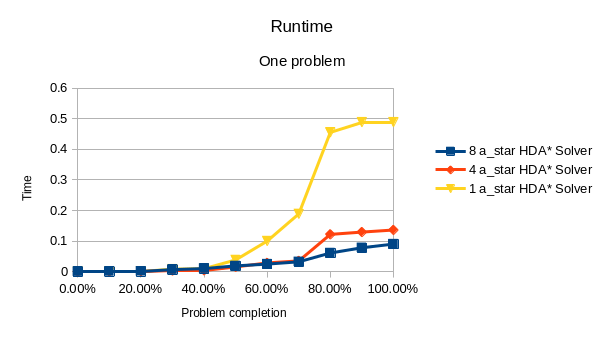
\includegraphics[width=\textwidth]{Media/Ch2/Runtime_One_Problem_Linear.png}
    \caption{Tiempo de ejecución de un único problema.}
    \label{fig:Runtime_One_Problem_Linear}
\end{figure}

Como se puede ver, el diagrama es de poca utilidad
para comparar algoritmos
debido a la complejidad del problema.
Para poder observar con mejor los resultados,
en las siguientes secciones se utilizan frencuentemente
gráficas con ejes verticales en escala logarítica
(figura \ref{fig:Runtime_One_Problem_Log}).

\begin{figure}[h]
    \centering
    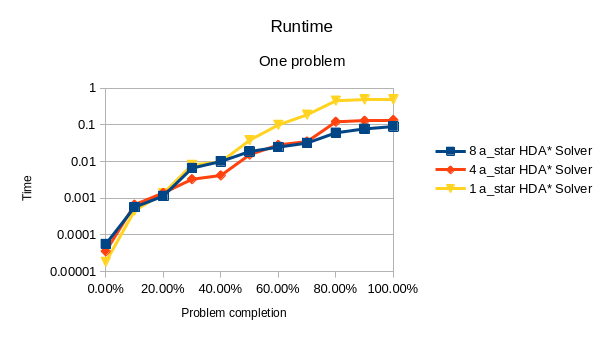
\includegraphics[width=\textwidth]{Media/Ch2/Runtime_One_Problem_Log.png}
    \caption{Tiempo de ejecución de un único problema (escala logarítmica).}
    \label{fig:Runtime_One_Problem_Log}
\end{figure}

Estas observaciones verifican que la complejidad del problema
a resolver es factorial, como era de esperar.

\begin{notebox}
    Este capítulo contiene diversas gráficas de las métricas obtenidas,
    obsérvese con detalle la escala utilizada en el eje de ordenadas de cada una
    ya que en algunos casos será logarítmica.
\end{notebox}

\subsection{Comparativa de heurísticos}
\index{Resultados!Heurísticos}

\subsubsection{Cotas Inferior v. Superior}

Como ya se discutió en la sección sobre optimización (\ref{ssec:Heuristicos}),
existen varias implementaciones de la función heurística que da al algoritmo
A* su particular comportamiento de ir `dirigido' hacia la solución.
En esta investigación se han implementado dos heurísticos:
uno de ellos es una cota inferior del coste restante mientras que
el otro es una cota superior.
El heurístico de cota inferior busca una solución que se acerque a la óptima lo máximo posible
mientras que el de cota superior busca la solución priorizando la velocidad del algoritmo.
A continuación se comparan los heurísticos utilizando el
$50\percentsign$ del conjunto \lstinline{abz5.csv} (5x5x10).

En primer lugar se observa que existe un limitado número de soluciones
propuestas, las más comunes siendo también las más bajas: 452 y 472.
Respecto al tiempo de ejecución, las pruebas que utilizan el heurístico rápido
reducen el tiempo de ejecución en varias magnitudes.

Aquellas implementaciones con sincronización (que retornan siempre el mismo resultado)
muestran una mayor precisión que aquellas que no (FCFS y HDA*).
Los algoritmos sin sincronización no se deberían utilizar junto
al heurístico rápido ya que la pérdida en precisión no
compensa el \italic{speedup}.
En los algoritmos con sincronización sin embargo sí existen
argumentos para sopesar el uso del heurístico rápido ya que
la pérdida en precisión podría compensar con creces
el \italic{speedup}.

\begin{keynotebox}
    La principal conclusión de las siguientes observaciones es que
    el heurístico rápido puede ser considerado sólo cuando
    se utilizan algoritmos monohilo o
    con sincronización.
    Y siempre haciendo observaciones previas
    para comprobar que el tamaño del problema no es demasiado grande
    ya que a mayor el tamaño del problema, peores los resultados.
\end{keynotebox}

\begin{figure}[H]
    \begin{subfigure}{.5\textwidth}
        \begin{center}
            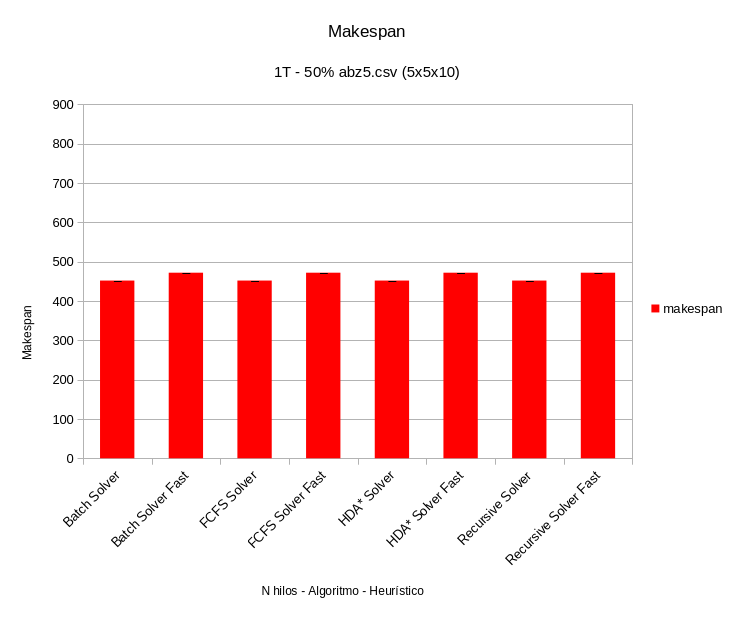
\includegraphics[width=\textwidth]{Media/Ch2/XMakespan_1_Heuristics.png}        
        \end{center}
        \subcaption{\italic{Makespan} heurísticos 1 hilo.}
        \label{fig:Heuristico1}
    \end{subfigure}
    \begin{subfigure}{.5\textwidth}
        \begin{center}
            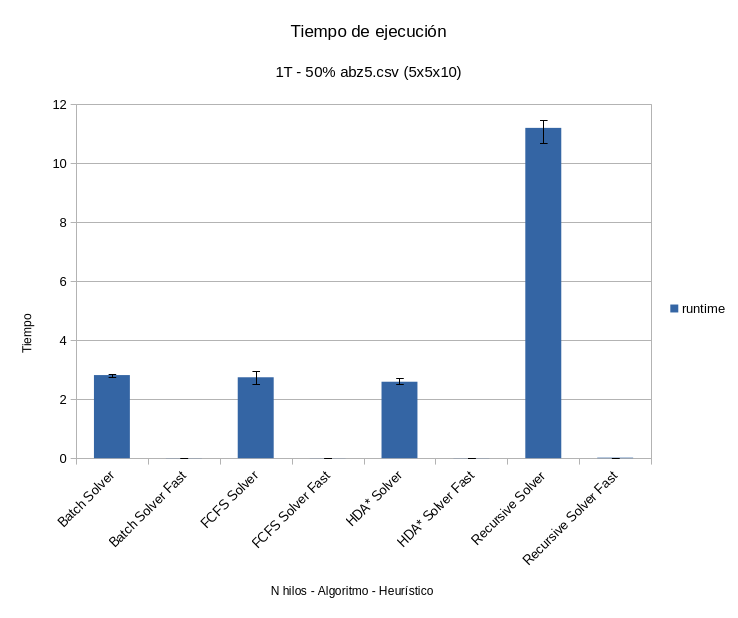
\includegraphics[width=\textwidth]{Media/Ch2/XRuntime_1_Heuristics.png}        
        \end{center}
        \subcaption{Tiempo de ejecución heurísticos 1 hilo.}
    \end{subfigure}
    \vskip\baselineskip
    \begin{subfigure}{.5\textwidth}
        \begin{center}
            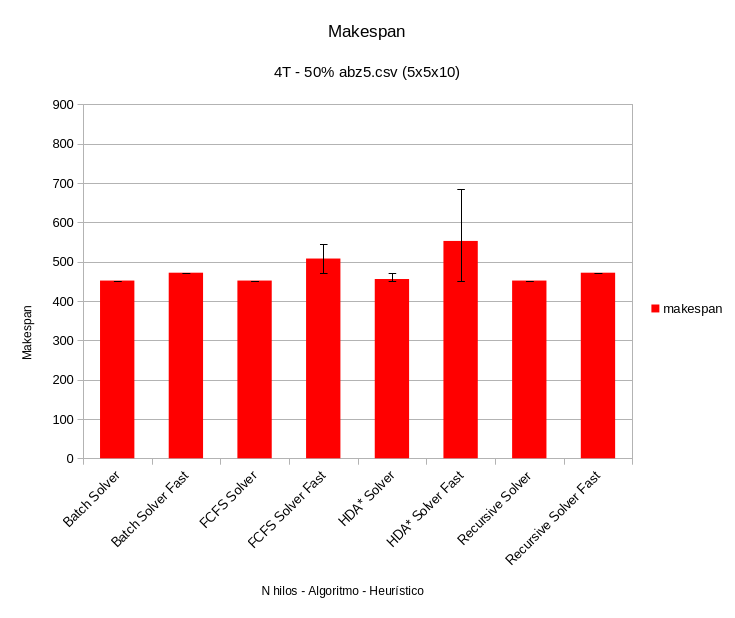
\includegraphics[width=\textwidth]{Media/Ch2/XMakespan_4_Heuristics.png}        
        \end{center}
        \subcaption{\italic{Makespan} heurísticos 4 hilos.}
        \label{fig:Heuristico4}
    \end{subfigure}
    \begin{subfigure}{.5\textwidth}
        \begin{center}
            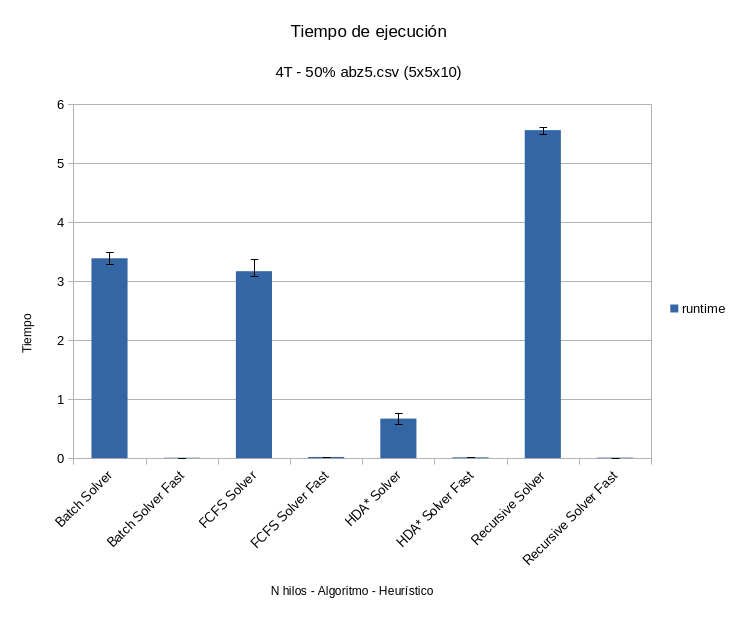
\includegraphics[width=\textwidth]{Media/Ch2/XRuntime_4_Heuristics.png}        
        \end{center}
        \subcaption{Tiempo de ejecución heurísticos 4 hilos.}
    \end{subfigure}
    \vskip\baselineskip
    \begin{subfigure}{.5\textwidth}
        \begin{center}
            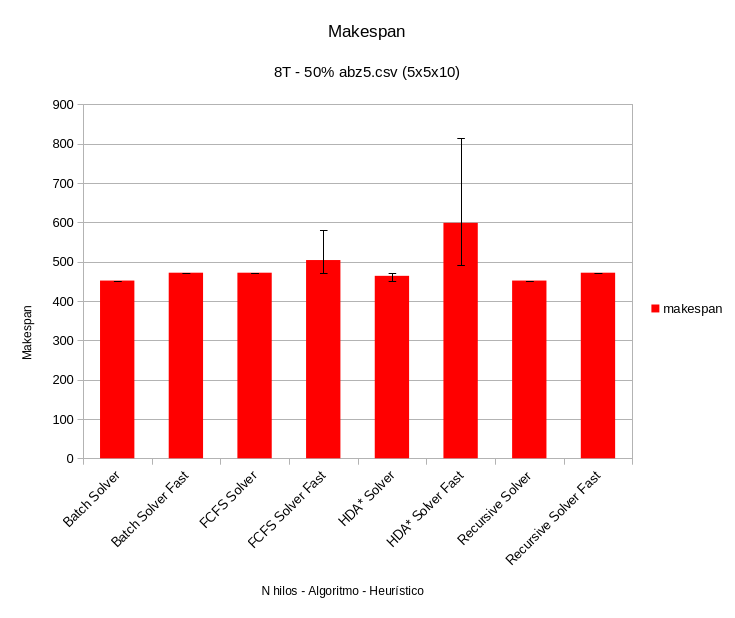
\includegraphics[width=\textwidth]{Media/Ch2/XMakespan_8_Heuristics.png}        
        \end{center}
        \subcaption{\italic{Makespan} heurísticos 8 hilos.}
        \label{fig:Heuristico8}
    \end{subfigure}
    \begin{subfigure}{.5\textwidth}
        \begin{center}
            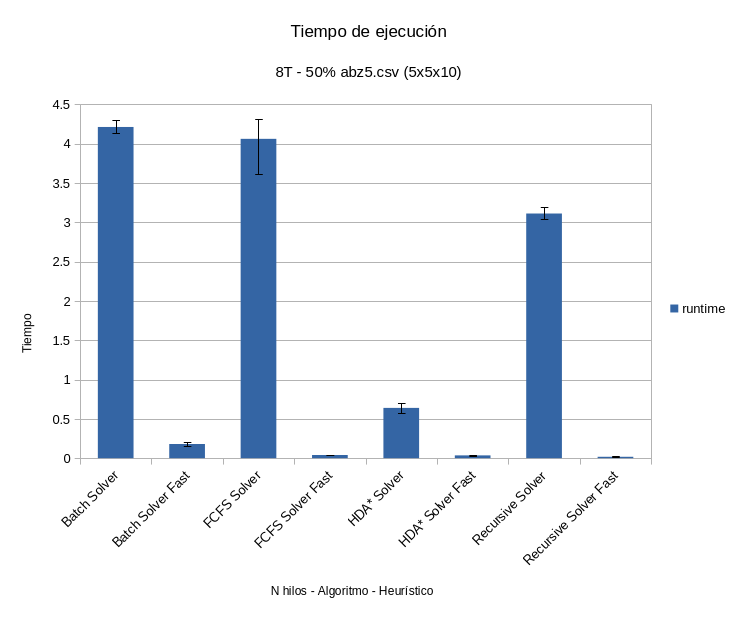
\includegraphics[width=\textwidth]{Media/Ch2/XRuntime_8_Heuristics.png}        
        \end{center}
        \subcaption{Tiempo de ejecución heurísticos 8 hilos.}
    \end{subfigure}
    \caption{Métricas de heurísticos.}
\end{figure}

Analizandolas por separado, las ejecuciones que utilizan el heurístico lento
retornaron siempre 452 o 472, los dos mejores resultados y se vieron
beneficiadas por el uso de varios hilos.
Por otro lado, las ejecuciones que utilizan el heurístico rápido
sólo retornaron 452 o 472 en algunas instancias y no se vieron
beneficiadas por el uso de varios hilos
(Véase figuras \ref{fig:Heuristico8}, \ref{fig:Heuristico4} y \ref{fig:Heuristico1}).

Sería razonable suponer que el heurístico rápido
sí se vería beneficiado por el paralelismo si el tamaño del
problema fuese lo suficientemente grande.
Para comprobar esta hipótesis, se ha creado un conjunto
con un tamaño mucho mayor (70x10x10) y se ha obtenido el \italic{speedup}.

Además, se puede observar una clara tendencia en los resultados que utilizan
el heurístico rápido. A menor número de hilos, mejor \italic{makespan} retornan.

\begin{figure}[h]
    \centering
    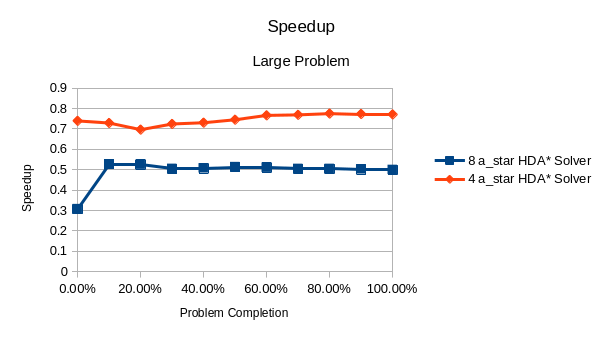
\includegraphics[width=\textwidth]{Media/Ch2/Speedup_Large_Problem.png}
    \caption{\italic{Speedup} en un problema de gran tamaño.}
    \label{fig:Speedup_Large_Problem}
\end{figure}

La gráfica (\ref{fig:Speedup_Large_Problem}) muestra que incluso en un problema de mayor tamaño
la versión monohilo es más rápida que las multihilo.
Esta investigación no ha podido encontrar un conjunto de datos
en el que utilizando el heurístico rápido valga la pena el paralelismo.
No obstante, se ha observado que a medida que el tamaño
del problema incrementa, el \italic{speedup} también se ve incrementado
por lo que si se supone que la tendencia del \italic{speedup}
se mantiene, sería razonable suponer que existe un tamaño de
problema donde sí vale la pena utilizar varios hilos y 
el heurístico rápido.

Se deja también constancia de que las pruebas ejecutadas indican que
el error cometido por el heurístico rápido incrementa proporcionalmente
con el tamaño del problema.
En las pruebas que utilizaron conjuntos de datos de 6x6x10,
el error se encontraba entre 20 y 50, mientras que en
conjuntos de datos de 70x10x10, el error se podría encontrar
en los miles.
Por ello, el heurístico rápido se podría considerar únicamente para
resolver problemas de menor tamaño e incluso en esos casos
se debería tener en cuenta su falta de precisión.

\begin{notebox}
    A menos que se indique lo contrario,
    las pruebas ejecutadas en esta investigación utilizan el heurístico de
    cota inferior ya que es el que retorna resultados óptimos.
\end{notebox}

\subsubsection{Random Solver}

El heurístico rápido obtiene resultados cuya calidad es razonable
únicamente cuando se tiene en cuenta la velocidad con la que
los obtiene.
Se ha implementado un algoritmo (no A*) que resuelve
el problema del JSP de forma aleatoria (Anexo \ref{sec:RandomSolver}),
esto es, selecciona una tarea cualquiera y la introduce en el plan.
Como el nombre del \italic{solver} indica, la planificación
que retorna este algoritmo es aleatoria.
Utilizamos estos resultados para criticar el \italic{makespan}
de una de las peores lecutras,
la del heurístico rápido en el algoritmo HDA* con cuatro hilos.

\begin{figure}[h]
    \centering
    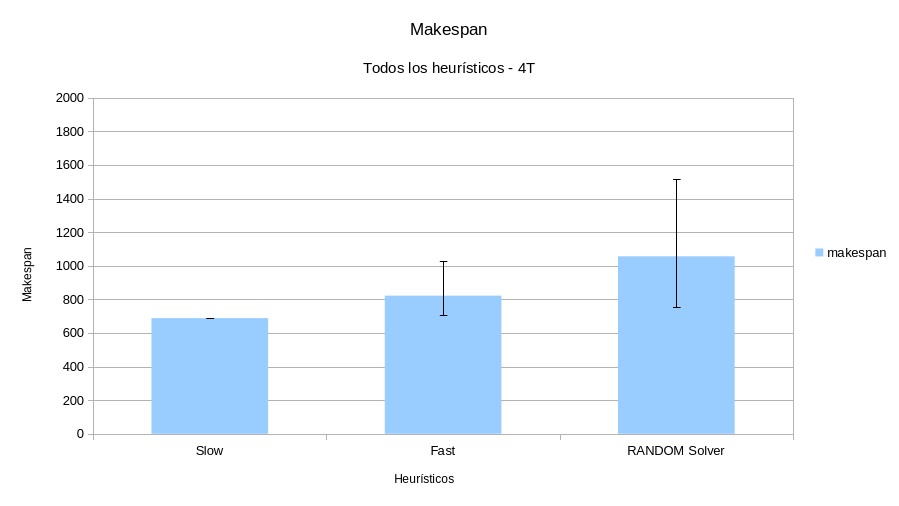
\includegraphics[width=\textwidth]{Media/Ch2/Makespan_Random_Solver.png}
    \caption{\italic{Makespan} de diferentes heurísticos}
    \label{fig:MakespanRandomSolver}
\end{figure}

La figura \ref{fig:MakespanRandomSolver} muestra el \italic{makespan}
del heurístico óptimo (el lento), el rápido y el obtenido
por el Random Solver.
Adicionalmente, se muestran también los \italic{makespan}
máximo y mínimo obtenidos por cada uno de ellos.

Como se puede ver en el diagrama, el heurístico rápido obtiene mejores
resultados que el Random Solver y más importantemente tiene un
margen de error mucho menor.
Entonces, aunque los resultados del heurístico rápido no
sean óptimos, son mejores que crear una planificación aleatoria.

\pagebreak
\subsubsection{Dijkstra}
\index{Resultados!Dijkstra}
\label{sec:ComparativaDijkstra}

Como se indicó brevemente al inicio de este documento (Subsección \ref{ssec:AlgoritmoA*}),
el algoritmo A* es una evolución del de Dijkstra
donde la principal diferencia es la inclusión de una función
heurística utilizada para seleccionar el siguiente nodo a explorar.
Entonces, se podría decir que el algoritmo de Dijkstra es una
versión particular del algoritmo A* donde la función heurística
retorna siempre 0.

En esta subsección se ha estudiado el rendimiento del algoritmo de Dijkstra
y los diferentes A* utilizando el heurístico de cota inferior,
que retorna resultados óptimos a cambio de un mayor tiempo de ejecución.

La principal conclusión obtenida de las siguientes observaciones 
(Figura \ref{fig:Speedup_Dijkstra}) es que el \italic{speedup}
del algoritmo A* frente a Dijkstra
es tan grande que incluso resulta complicado realizar pruebas.
Esto se debe a que los conjuntos de datos que se pueden
resolver utilizando Dijkstra en un tiempo razonable son resueltos
en microsegundos por A* y los que son resueltos en un tiempo
razonable por A* requerirían meses de ejecución para resolverlos
utilizando Dijkstra
\footnote{
    Es recomendable evitar extraer conclusiones de observaciones cuyo tiempo de ejecución es muy reducido.
    Existe un gran número de variables (cambios de contexto, fallos de caché, interrupciones del OS)
    que pueden afectar al tiempo de ejecución de un algoritmo,
    desvirtuando la medición.
}.

\begin{notebox}
    Nótese que el \italic{speedup} entre A* (utilizando el heurístico lento)
    y Dijkstra supera 8000 en todos los casos.
    Sabiendo que el heurístico lento es más lento que el heurístico rápido,
    se conoce por la propiedad transitiva que Dijkstra es más lento
    que el heurístico rápido.

    Tratar de hacer pruebas con el objetivo de calcular Dijkstra con el heurístico
    rápido retornaría una diferencia de tiempo de tal magnitud que sería
    imposible comprender la diferencia entre ambos,
    más aún tratar de representarlo en una gráfica.
\end{notebox}

\begin{figure}[h]
    \centering
    %\includesvg{./Media/Ch2/Speedup_Dijkstra.svg}
    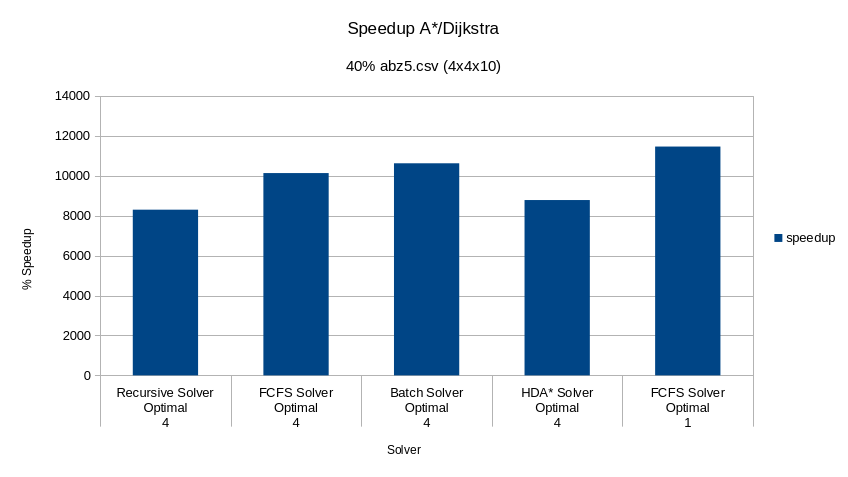
\includegraphics[width=\linewidth]{Media/Ch2/Speedup_Dijkstra.png}
    \caption{\italic{Speedup} de A* frente a Dijkstra}
    \label{fig:Speedup_Dijkstra}
\end{figure}

Como era de esperar, el rendimiento de las implementaciones A*
es notablemente superior al de Dijkstra en lo que corresponde
a tiempo de ejecución.
El gráfico anterior muestra que como poco el algoritmo A*
tiene un \italic{speedup} de 8000 frente a Dijkstra
en el conjunto de datos estudiado.

Las ejecuciones de Dijkstra han sido capaces
de obtener un \italic{makespan} mejor que
las implementaciones sin sincronización de A*.
El algoritmo de Dijkstra explorará todos los
nodos posibles hasta obtener una solución óptima
mientras que el A* simplemente explorará nodos
hasta que se cumpla la condición de salida
\footnote{En este caso que todas las tareas estén planificadas}.

El algoritmo A* es completo, retornará una solución al problema
siempre y cuando exista al menos una.
Esto no implica que sus resultados sean siempre óptimos
(A diferencia de Dijkstra, cuyos resultados sí lo son).
Que A* retorne soluciones óptimas o no depende de la función heurística
encargada de calcular el coste H.
Si la función heurística subestima el coste H real
(es cota inferior del coste H real)
entonces A* retornará la solución óptima.
En otro caso, A* retornará una solución que puede
ser la óptima.

De cualquier forma, las funciones heurísticas no son
categorizables en una u otra clase,
más bien se trata de un espectro.
Las funciones heurísticas que subestimen
el coste H real se denominan `optimistas'
mientras que las que lo igualan o sobreestiman
se denominan `pesimistas'.

\vspace{4em}

\begin{keynotebox}
Las funciones optimistas retornarán los resultados óptimos
pero requerirán un mayor tiempo de ejecución ya que
se verán obligadas a explorar un mayor número de nodos
mientras que las pesimistas no tienen por qué retornar un
resultado óptimo y tendrán una mayor velocidad porque
no explorarán tantas posibilidades.
\end{keynotebox}

\pagebreak

Al extremo de las funciones optimistas
se encuentra el algoritmo de Dijkstra
cuyo heurístico retorna siempre 0
(no hay coste más bajo) y
al extremo de las funciones pesimistas se podría encontrar la siguiente
función (\ref{eq:HeuristicoPesimista})
donde $J$ es el número total de trabajos, $T$ el de tareas y $D_{i,j}$
la duración de la tarea $j$ del trabajo $i$.

\begin{figure}[h]
    $$
    cost_h = \sum_{j=0}^{J}{
        \sum_{t=0}^{T}{
            D_{j,t}
        }
    }
    $$
    \caption{Función heurística pesimista}
    \label{eq:HeuristicoPesimista}
\end{figure}

Una función que calcula el sumatorio de todas las duraciones
de las tareas restantes por planificar.
Este heurístico sería lo equivalente a planificar
que cada tarea se ejecute una a una de forma
que sólo un trabajador se encuentra activo mientras
el resto esperan (aunque puedan hacer tareas de forma paralela).

En algún punto intermedio entre estos dos extremos
se encontraría el heurístico óptimo utilizado
en la mayoría de las pruebas de esta investigación,
pero es difícil de saber si se acerca más
a los algoritmos optimistas o pesimistas.
La principal dificultad de implementar el algoritmo A*
es entonces decidir una función heurística
que sea lo suficientemente pesimista para retornar resultados óptimos
pero no tan pesimista que explore demasiadas alternativas.

\pagebreak
\subsection{Comparativa de algoritmos}
\index{Resultados!Comparativa de algoritmos}

\subsubsection{Monohilo}

Como es de esperar, el rendimiento monohilo de todas
las implementaciones es el mismo.
Todas las implementaciones están diseñadas de forma
que al ser ejecutadas con un sólo hilo
el algoritmo sea el A* básico.

\begin{figure}[h]
    \begin{center}
        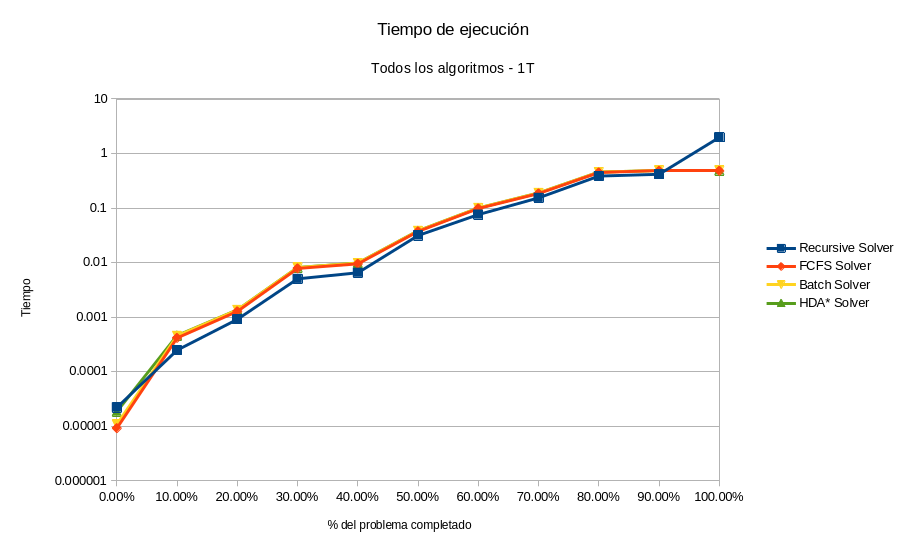
\includegraphics[width=\textwidth]{Media/Ch2/Runtime_All_Algorithms_1.png}
    \end{center}
    \caption{Tiempo de ejecución de todos los algoritmos (1 hilo).}
    \label{fig:MetricasSinglethread}
\end{figure}

\begin{figure}[h]
    \begin{subfigure}{.5\textwidth}
        \begin{center}
            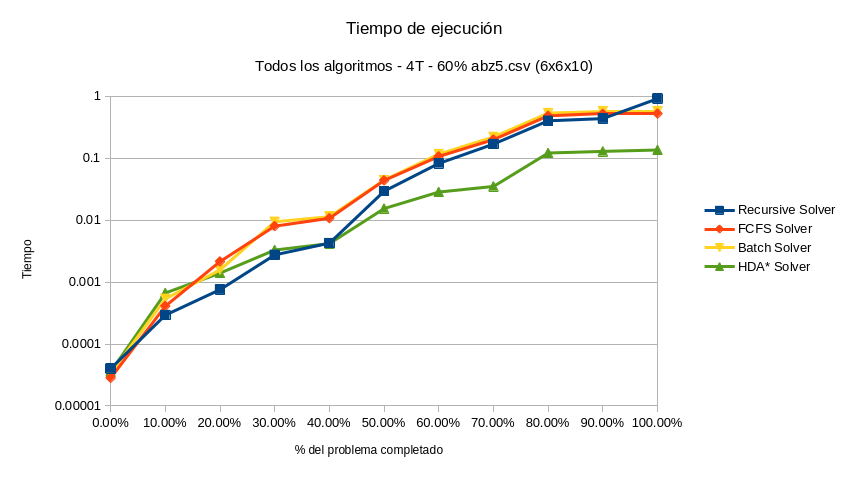
\includegraphics[width=\textwidth]{Media/Ch2/Runtime_All_Algorithms_4.png}
            \subcaption{Tiempo de ejecución de todos los algoritmos (4 hilos).}
        \end{center}
    \end{subfigure}
    \begin{subfigure}{.5\textwidth}
        \begin{center}
            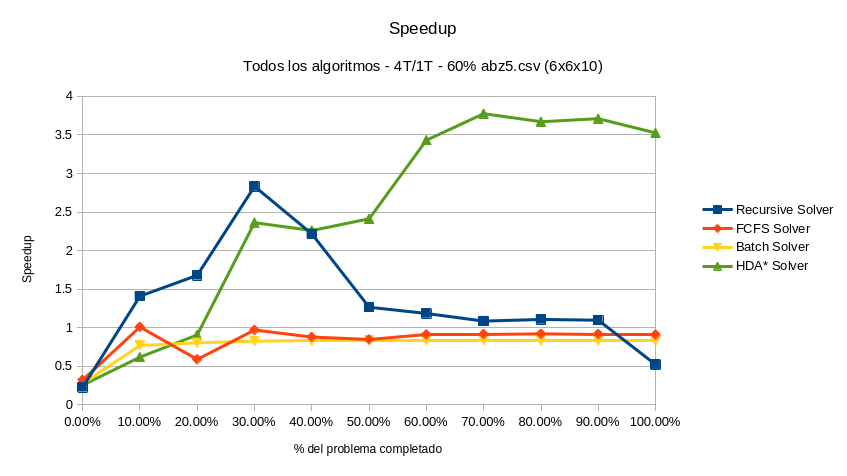
\includegraphics[width=\textwidth]{Media/Ch2/Speedup_All_Algorithms_4.png}
            \subcaption{\italic{Speedup} de todos los algoritmos (4 hilos).}
        \end{center}
    \end{subfigure}
    \caption{Métricas con 4 hilos.}
    \label{fig:Metricas4Thread}
\end{figure}

\pagebreak
\subsubsection{Con sincronización: Batch y Recursive}

Se observa el rendimiento de los algoritmos con sincronización entre hilos:
Batch y Recursive solver.
Al tener sincronización estos algoritmos retornan siempre la misma solución
para el mismo problema.

A modo de recordatorio:
\begin{itemize}[itemsep=0.25px]
    \item Batch solver: En cada iteración se exploran los mejores nodos conocidos.
    \item Recursive solver: Se resuelve el algoritmo A* para cada sucesor del nodo inicial.
\end{itemize}

\begin{figure}[h]
    \begin{center}
        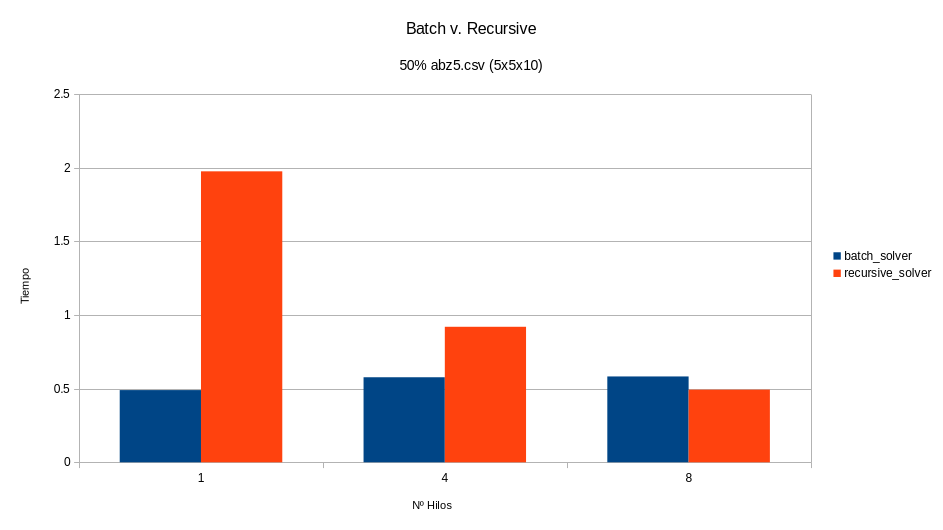
\includegraphics[width=\textwidth]{Media/Ch2/Runtime_BatchRecursive.png}
    \end{center}
    \caption{Tiempo de ejecución del algoritmos Batch y Recursive solvers.}
    \label{fig:BatchRecursive}
\end{figure}

En el caso general, el algoritmo Batch Solver sigue el mismo camino que
el A* monohilo. La principal diferencia es que al evaluar varios nodos
en cada iteración, puede encontrar un camino diferente al A* monohilo
que le lleve al resultado óptimo en menos tiempo.
No obstante, se ve obligado a destruir y crear al equipo de hilos
en cada iteración.
Además, al evaluar más nodos, el \lstinline{open_set} crece
más rápidamente, empeorando el principal cuello de botella
del algoritmo.
En las pruebas ejecutadas, estos sobrecostes
no compensan el posible ahorro de tiempo.

El algoritmo Recursive Solver resolverá el algoritmo A* monohilo $V$ veces
siendo $V$ el número de vecinos del nodo inicial.
Esto implica que en monohilo, el tiempo se ve multiplicado por $V$ veces.
Si se utilizan $N$ hilos pero hay $1.5 \times N$ vecinos del nodo inicial,
$N$ hilos ejecutarán el algoritmo A* y cuando hayan terminado, $N \over 2$
volverán a ejecutar otro A* para los nodos vecinos restantes.

Salvo en casos particulares, ninguna de estas estrategias supera el rendimiento
del algoritmo A* normal monohilo.

\subsubsection{Sin sincronización: FCFS y HDA*}

Se observa el rendimiento de los algoritmos sin sincronización entre hilos:
FCFS y HDA* solver.
Al no tener sincronización estos algoritmos pueden retornar diferentes
soluciones para el mismo problema.

A modo de recordatorio:
\begin{itemize}[itemsep=0.25px]
    \item FCFS: Los hilos exploran nodos tan pronto como estén disponibles en el \lstinline{open_set} compartido.
    \item HDA*: Igual que FCFS pero los nodos son asignados al \lstinline{open_set} privado de un hilo.
\end{itemize}

\begin{figure}[h]
    \begin{center}
        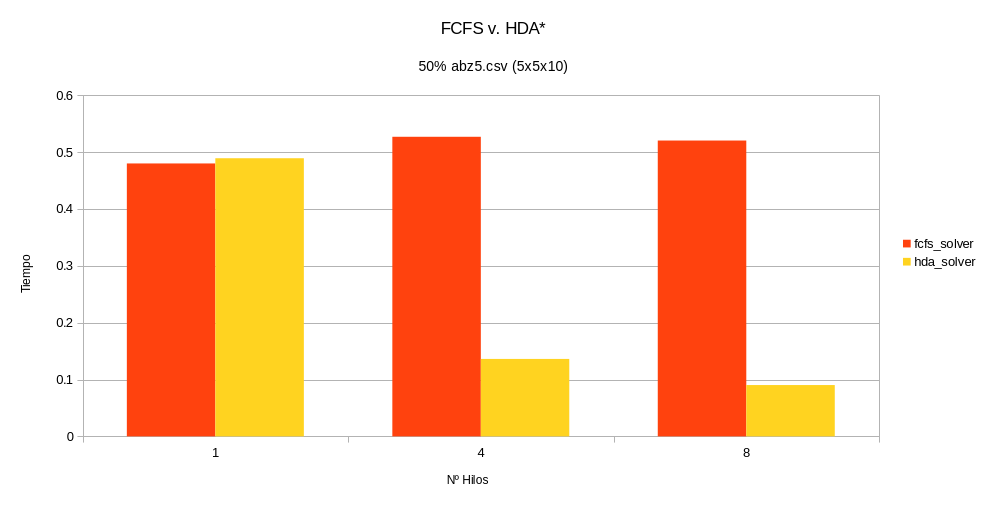
\includegraphics[width=\textwidth]{Media/Ch2/Runtime_FCFSHDA.png}
    \end{center}
    \caption{Tiempo de ejecución del algoritmos FCFS y HDA* solvers.}
    \label{fig:FCFSHDA}
\end{figure}

El algoritmo FCFS tiene prácticamente las mismas virtudes y defectos que el Batch solver.
Tiene una mayor posibilidad de encontrar el camino óptimo en menos tiempo
pero explora más nodos e incrementa el tamaño del \lstinline{open_set}
reduciendo su rendimiento.

El algoritmo HDA* sin embargo parece tener lo mejor de ambos mundos.
Por un lado explora una mayor cantidad de nodos
por lo que puede encontrar el camino óptimo en menos tiempo
pero distribuye los nodos descubiertos en diferentes \lstinline{open_set},
reduciendo los efectos del cuello de botella.
Esto es, la reducción del cuello de botella es directamente proporcional
al número de hilos que estén trabajando en el problema
\footnote{Si el tamaño del problema es lo suficientemente grande.}.

\subsubsection{Todos los algoritmos}

Al utilizar cuatro hilos (figura \ref{fig:Metricas4Thread}), se puede comenzar a ver una diferencia clara
en el rendimiento del algoritmo HDA*, que obtiene un \italic{speedup}
de casi 4.

\begin{figure}[h]
    \begin{subfigure}{.5\textwidth}
        \begin{center}
            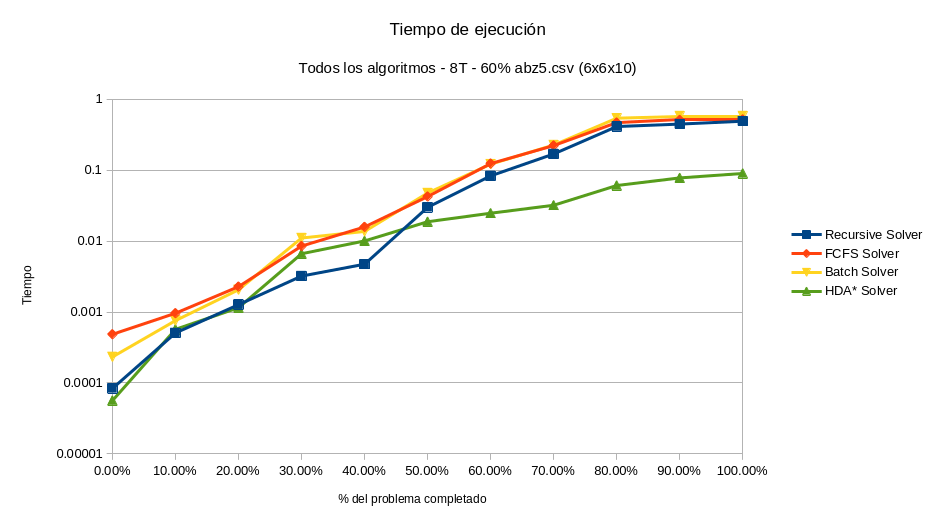
\includegraphics[width=\textwidth]{Media/Ch2/Runtime_All_Algorithms_8.png}
            \subcaption{Tiempo de ejecución de todos los algoritmos (8 hilos).}
        \end{center}
    \end{subfigure}
    \begin{subfigure}{.5\textwidth}
        \begin{center}
            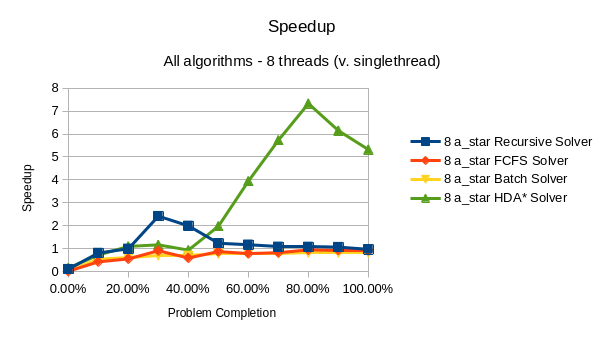
\includegraphics[width=\textwidth]{Media/Ch2/Speedup_All_Algorithms_8.png}
            \subcaption{\italic{Speedup} de todos los algoritmos (8 hilos).}
        \end{center}
    \end{subfigure}
    \caption{Métricas con 8 hilos.}
    \label{fig:Metricas8Thread}
\end{figure}

Al utilizar ocho hilos (figura \ref{fig:Metricas8Thread}),
el algoritmo HDA* incrementa aún más su diferencia
en el tiempo de ejecución con respecto al resto de algoritmos,
aunque esta vez el \italic{speedup} fluctua más.
De cualquier forma, parece ser capaz de alcanzar casi
el máximo \italic{speedup} posible para este número de hilos (8).

La principal conclusión de estas observaciones es que
(al menos en los conjuntos de datos observados),
en casos generales,
el paralelismo sólo es rentable si se implementa el HDA*.
En el resto de casos, el paralelismo sólo sirve para
gastar núcleos y ciclos de CPU a cambio de nada.

\begin{notebox}
    En la inmensa mayoría de observaciones realizadas,
    el algoritmo Batch Solver
    ha sido capaz de resolver el $30\percentsign$ del problema
    en menos tiempo que cualquier otro algoritmo.
    Esta reducción de tiempo se debe a que este algoritmo ejecuta el A*
    tantas veces como hilos haya disponibles de forma simultánea,
    facilitando la obtención de planificaciones profundas más rápido. 
    En otras palabras, el algoritmo es más veloz al iniciar el problema
    pero es más lento al final.
\end{notebox}

\pagebreak
\subsection{FPGA}

Se han tomado varias mediciones del algoritmo monohilo corriendo en la FPGA.
Los resultados muestran que la implementación de la FPGA es más lenta
en todos los casos salvo el Recursive Solver.
Esto es comprensible ya que el Recursive Solver debe ejecutar varias
veces el algoritmo cuando el número de hilos es inferior al
número de nodos vecinos del nodo inicial.

\begin{figure}[h]
    \begin{center}
        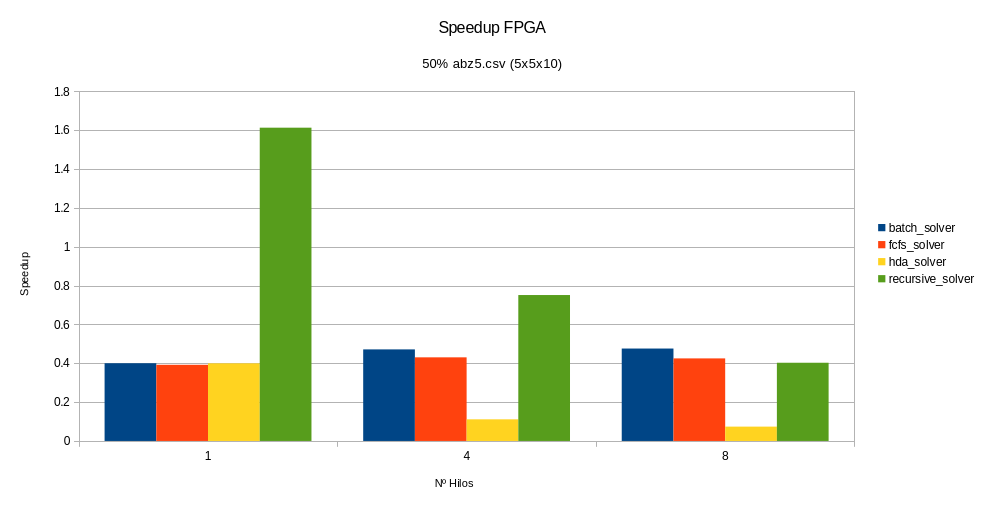
\includegraphics[width=\textwidth]{Media/Ch2/Speedup_FPGA.png}
        \caption{\italic{Speedup} de la FPGA frente al resto de algoritmos.}
        \label{fig:SpeedupFPGA}
    \end{center}
\end{figure}

La gráfica \ref{fig:SpeedupFPGA} muestra el \italic{speedup} del algoritmo
en la FPGA respecto al resto de implementaciones monohilo y paralelas.
Se ha observado también el comportamiento de este algoritmo
a lo largo de diferentes tamaños de problema con el objetivo de hallar el
máximo tamaño que se puede resolver en un tiempo razonable.

Los resultados de \italic{speedup} de todas estas mediciones son similares
a la gráfica anterior por lo que se han omitido.
Las ejecuciones en CPU han sido capaces de resolver en un tiempo
razonable problemas de tamaño 6x6x10 generalmente en menos de una hora, los problemas
de 7x7x10 tardan varias horas o días en función de cómo de fácil sea hallar
el camino solución.
La FPGA por otro lado ha sido capaz de resolver problemas de tamaño 4x4x10
con relativa facilidad en menos de una hora pero se estanca en algunos
problemas de tamaño 5x5x10.

\begin{keynotebox}
    Con la síntesis hecha en esta investigación,
    el algoritmo en FPGA tarda en resolver un problema
    de tamaño 4x4x10 lo mismo que una CPU tarda
    en resolver un problema 6x6x10.
\end{keynotebox}

Lo más seguro es que la FPGA sea capaz de superar en algún caso el rendimiento
en CPU dados el algoritmo, implementación y problema adecuados.
Esto no ha sucedido muy probablemente por falta de conocimiento y práctica
a la hora de escribir código transpilable con HLS.

\pagebreak
\subsection{Casos particulares}
\index{Resultados!Casos particulares}

Vistos los resultados anteriores
se podrían dar como obsoletas algunas de las versiones
paralelas por ofrecer muy pocas mejoras frente a otras
versiones monohilo.
No obstante, existen casos particulares del problema
donde estas versiones fácilmente descartables
podrían presentar una solución mucho más interesante.

Estos casos particulares generalmente involucran
la posibilidad de que la población de nodos sea
repartida entre los diferentes hilos de forma
que cada uno tenga una sección parcial o totalmente
independiente del resto.
A continuación se presentan algunos de estos casos.

\subsubsection{Varios estados iniciales}
\index{Resultados!Casos particulares!Varios estados iniciales}

Si el problema a resolver tiene varios estados iniciales
sería posible asignar cada estado a un hilo (o grupo de hilos)
de forma que cada uno busque una solución desde su estado inicial.

\subsubsection{Estados solución intermedios}
\index{Resultados!Casos particulares!Estados solución intermedios}

Si se conoce algún nodo intermedio de la solución
sería posible dividir el problema en dos,
de forma que un hilo resuelva una de las partes
\footnote{Si existiese más de un nodo intermedio conocido,
el problema se podría seguir subdividiendo entre más hilos.}.
Por ejemplo, si del problema se conocen el nodo inicial $A$,
el final $E$ y los intermedios $B$, $C$ y $D$,
la solución se podría obtener repartiendo el
trabajo entre 4 hilos diferentes:
\begin{enumerate}[start=0, itemsep=0.25px]
    \item Hilo 0: Resolver camino desde nodo $A$ hasta $B$.
    \item Hilo 1: Resolver camino desde nodo $B$ hasta $C$.
    \item Hilo 2: Resolver camino desde nodo $C$ hasta $D$.
    \item Hilo 3: Resolver camino desde nodo $D$ hasta $E$.
\end{enumerate}

\Chapter{Conclusiones}{Observaciones y Trabajos futuros}

\section{El algoritmo A*}

El algoritmo A* es de gran utilidad en un gran abanico de ámbitos.
Realmente, se trata de un algoritmo apto para cualquier problema
que esté formado por un grupo de nodos relacionables entre ellos
dodne se quiera buscar una ruta entre ellos desde un inicio hasta
un fin.

Desde el punto de vista más abstracto sólo existen tres funciones
dependientes del problema en particular mientras que el resto
del algoritmo sirve para cualquier problema:

\begin{itemize}[itemsep=0.25px]
    \item Dado un nodo conocer si es el objetivo o no.
    \item Dado un nodo conocer sus vecinos.
    \item Dado un nodo conocer sus costes G y H.
\end{itemize}

\section{Principal cuello de botella}

Existen tres principales operaciones necesarias para
ejecutar el algoritmo A*:

\begin{itemize}[itemsep=0.25px]
    \item Obtención del siguiente nodo a explorar del \lstinline{open_set}.
    \item Obtención de vecinos de un nodo.
    \item Inserción de vecinos en el \lstinline{open_set}.
\end{itemize}

La obtención de vecinos de un nodo es un algoritmo dependiente del problema a resolver.
Con el diseño de estructuras de datos e implementación correctos es fácil
minimizar el coste de esta operación.

La obtención del siguiente nodo a explorar del \lstinline{open_set}
puede ser resuelta en O(1) por cualquier desarrollador con un conocimiento
básico sobre estructuras de datos como listas enlazadas.

La inserción de vecinos en el \lstinline{open_set} es más complicada
ya que está estrechamente relacionada con la obtención del siguiente nodo
a explorar.
Generalmente el \lstinline{open_set} se implementará como una lista ordenada
de forma que el primer elemento sea el siguiente nodo a explorar.
Esto implica que los vecinos se deben introducir en orden,
insertando elementos en medio de la lista.
La operación de insertar elementos en medio de una lista suele ser
costosa.
En esta investigación se ha conseguido hacer en O(n) utilizando
una lista doblemente enlazada y un iterador que compara e inserta
en el mismo barrido.

Es posible reducir el coste computacional de insertar vecinos en el \lstinline{open_set},
pero esto implica un aumento en el coste de obtener el siguiente nodo a explorar.
Sería necesario diseñar una estructura de datos distinta para
reducir el coste computacional de una operación sin incrementar el de la otra.
Seguramente esta estructura de datos sea también más dependiente de la memoria
y como ya se ha visto en HDA*, el diseño de esta estructura debería
facilitar el uso de varios hilos.

El principal problema del \lstinline{open_set} es que la complejidad de sus operaciones
incrementa a medida que se añaden más nodos.
Es posible que otra forma de optimizar esta estructura se encuentre en hallar cómo
almacenar menos nodos en ella.

\section{Heurísticos}

Como ya se discutió en la sección comparativa con Dijkstra (\ref{sec:ComparativaDijkstra}),
el diseño de la función heurística es crucial para determinar si la implementación
del A* será admisible\footnote{Si retornará siempre el resultado óptimo.}
y el tiempo que requerirá para resolver el problema.

Ignorando el paralelismo, la decisión del diseño de la función heurística
es la principal clave que definirá el rendimiento y calidad de las soluciones
propuestas por el algoritmo.
Comprender las diferencias entre funciones optimistas y pesimistas
y ser capaz de hallar la función que retorne resultados óptimos en
el menor tiempo posible es el principal desafío de la implementación de este algoritmo.


%----------------------------------------------------------------------------------------
%	THESIS CONTENT - APPENDICES
%----------------------------------------------------------------------------------------

\appendix % Cue to tell LaTeX that the following "chapters" are Appendices

% Include the appendices of the thesis as separate files from the Appendices folder
% Uncomment the lines as you write the Appendices

%\include{Appendices/AppendixA}
\Chapter{Código Fuente}{}

\section{Chronometer}

\begin{lstlisting}[language=C++, caption=Clase Chronometer utilizada para tomar mediciones, label=lst:Chronometer]
class Chronometer
{
private:
    std::chrono::_V2::system_clock::time_point m_start_time;
    std::map<unsigned short, bool> m_goals;
    std::map<unsigned short, double> m_times;
    std::string m_solver_name;

public:
    Chronometer() : Chronometer(
        std::map<unsigned short, bool>(),
        "Unknown Solver") {}
    explicit Chronometer(
        const std::map<unsigned short, bool> &goals,
        std::string const &solver_name) : m_goals(goals),
                                          m_solver_name(solver_name) {}

    void start()
    {
        this->m_start_time = std::chrono::high_resolution_clock::now();
    }
    std::chrono::duration<double> time() const
    {
        return (
            std::chrono::high_resolution_clock::now() -
            this->m_start_time
        );
    }

    void process_iteration(const State &state);
    void log_timestamp(unsigned short goal, const State &state);
    void enable_goals();
    std::map<unsigned short, double> get_timestamps() const;
};
\end{lstlisting}

\section{Random Solver}
\label{sec:RandomSolver}

\begin{lstlisting}[language=C++, caption=Clase RandomSolver utilizada para resolver un problema aleatoriamente]
class RandomSolver : public AStarSolver
{
private:
    State get_random_next_state(const State &, std::mt19937 &) const;

public:
    RandomSolver() = default;
    ~RandomSolver() override = default;

    State solve(
        std::vector<std::vector<Task>>,
        std::size_t,
        Chronometer &) const override;

    std::string get_name() const override { return "RANDOM Solver"; };
};

State RandomSolver::solve(
    std::vector<std::vector<Task>> jobs,
    std::size_t n_workers,
    Chronometer &c) const
{
    const std::size_t nJobs = jobs.size();
    if (nJobs == 0)
        return State();
    const std::size_t nTasks = jobs[0].size();
    if (nTasks == 0)
        return State();
    if (n_workers == 0)
        n_workers = nTasks;

    std::random_device rd;
    std::mt19937 gen(rd());

    const auto startingSchedule = std::vector<std::vector<int>>(nJobs, std::vector<int>(nTasks, -1));
    const auto startingWorkersStatus = std::vector<int>(n_workers, 0);
    auto currentState = State(jobs, startingSchedule, startingWorkersStatus);

    while (!currentState.is_goal_state())
    {
        currentState = this->get_random_next_state(currentState, gen);
        c.process_iteration(currentState);
    }

    return currentState;
}

State RandomSolver::get_random_next_state(const State &currentState, std::mt19937 &gen) const
{
    std::vector<State> neighbors = currentState.get_neighbors_of();
    std::uniform_int_distribution<> dis(0, (int)neighbors.size() - 1);
    return neighbors[dis(gen)];
}
\end{lstlisting}

\section{Read and Cut}
\label{sec:ReadAndCut}

\begin{lstlisting}[
    language=C++,
    caption=Funciones utilizadas para leer y cortar conjuntos de datos
]
struct ReadTaskStruct
{
    unsigned int duration;
    std::vector<unsigned int> qualified_workers;
};

std::vector<std::vector<Task>> get_jobs_from_file(
    const std::string &filename
) {
    std::ifstream file(filename);
    std::string my_string;
    std::string my_number;
    std::vector<std::vector<ReadTaskStruct>> data;
    std::vector<std::vector<Task>> out;
    if (!file.is_open())
    {
        std::cerr << "Could not read file" << std::endl;
        file.close();
        return out;
    }
    while (std::getline(file, my_string))
    {
        std::stringstream line(my_string);
        data.emplace_back();
        bool is_worker = true;
        unsigned int qualified_worker = 0;
        while (std::getline(line, my_number, ';'))
        {
            if (is_worker)
            {
                qualified_worker = stoi(my_number);
                is_worker = false;
            }
            else
            {
                data[data.size() - 1].emplace_back();
                data[data.size() - 1][
                    data[data.size() - 1].size() - 1
                ].duration = stoi(my_number);
                data[data.size() - 1][
                    data[data.size() - 1].size() - 1
                ].qualified_workers = std::vector<unsigned int>(
                    1,
                    qualified_worker
                );
                is_worker = true;
            }
        }
    }
    for (std::size_t job_idx = 0; job_idx < data.size(); job_idx++)
    {
        out.emplace_back();
        const std::vector<struct ReadTaskStruct> currentJob = data[
            job_idx
        ];
        for (
            std::size_t task_idx = 0;
            task_idx < currentJob.size();
            task_idx++
        ) {
            const struct ReadTaskStruct currentTask = currentJob[
                task_idx
            ];
            unsigned int h_cost = 0;
            for (
                std::size_t unscheduled_task_idx = task_idx;
                unscheduled_task_idx < currentJob.size();
                unscheduled_task_idx++
            )
                h_cost += currentJob[unscheduled_task_idx].duration;
            out[job_idx].emplace_back(
                currentTask.duration,
                h_cost,
                currentTask.qualified_workers
            );
        }
    }
    file.close();
    return out;
}

std::vector<std::vector<Task>> cut(
    std::vector<std::vector<Task>> jobs,
    float percentage
) {
    percentage = percentage < 0 ? 0 : percentage;
    percentage = percentage > 1 ? 1 : percentage;
    const unsigned int jobs_to_keep = int(
        float(jobs.size()) * percentage
    );
    const unsigned int tasks_to_keep = int(
        float(jobs[0].size()) * percentage
    );
    std::vector<std::vector<Task>> new_jobs;

    for (unsigned int job_idx = 0; job_idx < jobs_to_keep; job_idx++)
    {
        new_jobs.emplace_back();
        for (
            unsigned int task_idx = 0;
            task_idx < tasks_to_keep;
            task_idx++
        )
            new_jobs[job_idx].push_back(jobs[job_idx][task_idx]);
    }

    return new_jobs;
}
\end{lstlisting}

\pagebreak
\section{Heurísticos}

\subsection{Slow - Óptimo}
\label{ssec:SlowOptimo}

\begin{lstlisting}[language=C++]
unsigned int State::calculate_h_cost() const
{
    std::vector<int> h_costs;
    for (size_t job_idx = 0; job_idx < this->m_jobs.size(); job_idx++)
    {
        h_costs.emplace_back(0);
        std::vector<Task> job = this->m_jobs[job_idx];
        for (size_t task_idx = 0; task_idx < job.size(); task_idx++)
            if (this->get_schedule()[job_idx][task_idx] == -1)
                h_costs[job_idx] += job[task_idx].get_duration();
    }
    auto max_element = std::max_element(h_costs.begin(), h_costs.end());
    return max_element == h_costs.end() ? 0 : *max_element;
}
\end{lstlisting}

\subsection{Fast}
\label{ssec:Fast}

\begin{lstlisting}[language=C++]
unsigned int State::calculate_h_cost() const
{
    unsigned int unscheduled_tasks_count = 0;
    for (std::size_t job_idx = 0; job_idx < this->m_jobs.size(); job_idx++)
        for (std::size_t task_idx = 0; task_idx < this->m_jobs[job_idx].size(); task_idx++)
            if (this->m_schedule[job_idx][task_idx] == -1)
                unscheduled_tasks_count += this->m_jobs[job_idx][task_idx].get_duration();
    return unscheduled_tasks_count; 
}
\end{lstlisting}

\pagebreak

\Chapter{Resultados y Métricas}{}
\chapter{Diagramas}{}

\section{Diagrama Pert}
\label{sec:Pert}

\begin{figure}[h]
    \begin{center}
        \begin{tikzpicture}[node distance=4cm]
            % \node (08) [dot, right of=06, xshift=4cm] {\lstinline{n_2}};
            % \draw [arrow] (01.south) to node [anchor=west] {\lstinline{pop()}} (04);
            % \draw [arrow] (04.south) to node [anchor=west] {\lstinline{process()}} (06);
            % \draw [arrow] (06.west) to [bend left] node [anchor=north] {\lstinline{neighbor_0}} (05);

            \node (A) [dot] {0, 0};

            \node (B) [dot, right of=A, above of=A] {2, 3};
            \node (C) [dot, right of=A, below of=A] {3, 3};

            \node (D) [dot, right of=B] {7, 8};
            \node (E) [dot, right of=C] {6, 6};

            \node (F) [dot, right of=D, below of=D] {9, 9};

            \draw [arrow] (A.east) to node [anchor=south east] {T00(2)} (B);
            \draw [arrow] (A.east) to node [anchor=north east] {T10(3)} (C);

            \draw [arrow] (B.east) to node [anchor=south] {T01(5)} (D);
            \draw [arrow] (C.east) to node [anchor=north] {T11(3)} (E);

            \draw [arrow] (D.east) to node [anchor=south west] {T02(1)} (F);
            \draw [arrow] (E.east) to node [anchor=north west] {T12(3)} (F);
        \end{tikzpicture}
    \end{center}
    \caption{Diagrama Pert ejemplo.}
    \label{fig:ExamplePert}
\end{figure}

\pagebreak
\section{Diagrama Gantt}
\label{sec:Gantt}

\begin{figure}[h]
    \begin{center}
        \begin{tikzpicture}[node distance=4cm]
            \node (T00) [dot] at (0, 12) {T00};
            \node (T01) [dot] at (0, 10) {T01};
            \node (T02) [dot] at (0, 8) {T02};

            \node (T10) [dot] at (0, 4) {T10};
            \node (T11) [dot] at (0, 2) {T11};
            \node (T12) [dot] at (0, 0) {T12};

            \node (00) [process, fill=yellow!60] at(4, 12) {0 - T00(2) - 2};
            \node (10) [process, fill=green!60] at(4, 4) {0 - T10(3) - 3};

            \node (01) [process, fill=green!60] at(8, 10) {3 - T01(5) - 8};
            \node (11) [process, fill=red!60] at(8, 2) {3 - T11(3) - 6};

            \node (02) [process, fill=red!60] at(12, 8) {8 - T02(1) - 9};
            \node (12) [process, fill=yellow!60] at(12, 0) {6 - T12(3) - 9};
        \end{tikzpicture}
    \end{center}
    \caption{Diagrama Gantt ejemplo.}
\end{figure}

\pagebreak
\section{Algoritmo A*}

\begin{figure}[h]
\begin{center}
\begin{tikzpicture}[node distance=2cm]
    \node (A) [startstop] {Inicio};

    \node (B) [process, right of=A, xshift=2cm] {
        Inicializar \lstinline{g_costs}, \lstinline{f_costs} y \lstinline{open_set}
    };

    \node (C) [decision, below of=B, yshift=-2cm] {
        ¿Se ha encontrado el objetivo?
    };

    \node (D) [startstop, right of=C, xshift=3.5cm] {
        Retornar
    };

    \node (E) [process, left of=C, xshift=-3.5cm] {
        Asignar el primer elemento de \lstinline{open_set}
        al nodo actual
    };

    \node (F) [process, below of=E, yshift=-0.5cm] {
        Calcular nodos vecinos del nodo actual
    };

    \node (G) [decision, below of=F, yshift=-1.5cm] {
        ¿Hay vecinos? 
    };
    
    \node (H) [process, below of=G, yshift=-2cm] {
        Calcular el coste G del sucesor actual
    };

    \node (I) [decision, right of=H, xshift=3.5cm] {
        ¿Es el mejor coste G que se conoce para este estado?
    };

    \node (J) [process, right of=I, xshift=3.5cm] {
        Guardar coste G y nodo en \lstinline{g_costs} y \lstinline{f_costs}
    };

    \node (K) [decision, above of=J, yshift=2cm] {
        ¿Existe el nodo en el \lstinline{open_set}?
    };

    \node (L) [process, left of=K, xshift=-3.5cm] {
        Insertar en \lstinline{open_set}
    };

    \draw [arrow] (A) -- (B);
    \draw [arrow] (B) -- (C);
    \draw [arrow] (C) -- node [anchor=north] {Sí} (D);
    \draw [arrow] (C) -- node [anchor=north] {No} (E);
    \draw [arrow] (E) -- (F);
    \draw [arrow] (F) -- (G);
    \draw [arrow] (G) -- node [anchor=north west] {No} (C);
    \draw [arrow] (G) -- node [anchor=east] {Sí} (H);
    \draw [arrow] (H) -- (I);
    \draw [arrow] (I) -- node [anchor=north east] {No} (G);
    \draw [arrow] (I) -- node [anchor=north] {Sí} (J);
    \draw [arrow] (J) -- (K);
    \draw [arrow] (K) -- node [anchor=north east] {No} (C);
    \draw [arrow] (K) -- node [anchor=north] {Sí} (L);
    \draw [arrow] (L) -- (G);
\end{tikzpicture}
\end{center}
\caption{Representación del algoritmo A*}
\label{fig:AlgoritmoA*}
\end{figure}


%----------------------------------------------------------------------------------------
%	BIBLIOGRAPHY
%----------------------------------------------------------------------------------------

\nocite{*}
\printbibliography[heading=bibintoc]

%----------------------------------------------------------------------------------------

\addchaptertocentry{Índice alfabético}
\printindex

\end{document}  
